%-----------------------------------------------------------------------------%
\chapter{IMPLEMENTASI DAN PENGUJIAN}
%-----------------------------------------------------------------------------%

%
\vspace{4.5pt}
\noindent Pada bab ini akan menjelaskan mengenai proses implementasi dan pengujian terhadap sistem yang telah dibangun berdasarkan penjelasan pada bab sebelumnya.\\

\section{Lingkungan Implementasi}
\noindent Pada lingkungan implementasi, akan dijelaskan mengenai perangkat yang digunakan dalam proses pembangunan sistem baik dari perangkat keras maupun perangkat lunak yang digunakan.\\

\subsection{Spesifikasi Perangkat Keras}
\noindent Spesifikasi dari perangkat keras yang digunakan dalam pembangunan aplikasi adalah sebagai berikut:
\begin{enumerate}
\item \textit{Laptop} ASUS A442UQ
\item \textit{Processor} Intel Core i7-7500U CPU @ 2.7GHz
\item \textit{Hard Disk} kapasitas 1TB
\item RAM 16GB\\
\end{enumerate}

\subsection{Lingkungan Perangkat Lunak}
\noindent Spesifikasi dari perangkat lunak yang digunakan dalam pembangunan aplikasi adalah sebagai berikut:
\begin{enumerate}
\item Sistem Operasi Windows 10 Home 64 bit.
\item Netbeans IDE 8.2
\item Java Development Kit (JDK) 1.8.0{\_}161
\item \textit{Library} OpenCV 3.4.6\\
\end{enumerate}

%\subsection{Penjelasan \textit{Dataset}}
%\noindent Pada implementasi digunakan dua buah \textit{dataset} yaitu \textit{Clothing Store} dan \textit{Outdoor}. Seperti yang telah dijelaskan pada bab 2, 80\% citra dari \textit{dataset Clothing Store} akan digunakan untuk pembelajaran dan 20\% citra lainya untuk pengujian. Sementara \textit{dataset Outdoor} yang terdiri atas 3 buah folder yaitu 31, 54, dan 56, di mana seluruh citra pada folder 56 untuk data belajar, lalu folder 31 dan folder 54 untuk data uji. Pada masing-masing \textit{dataset} didapatkan masing-masing citra positif yaitu berisi manusia sesuai dengan berkas \textit{ground truth} sedangkan citra negatif yaitu berisi selain manusia didapatkan secara acak yang tidak berpotongan dengan daerah citra manusia. Ukuran dari citra negatif adalah 65 $\times$ 80 piksel. Rincian dari jumlah citra, citra positif, dan citra negatif dapat dilihat pada tabel \ref{tbl:rincianDataset}.
%\begingroup
%\setlength{\LTleft}{-20cm plus -1fill}
%\setlength{\LTright}{\LTleft}
%\begin{small}
%\begin{longtable}{|c|c|c|c|c|c|c|}
%\caption{Rincian \textit{Dataset} untuk Implementasi}
%\label{tbl:rincianDataset}
%\endhead
%\hline
%\textit{\textbf{Dataset}}			& \textbf{Folder}			& \textbf{Keterangan}	& \textbf{Citra Belajar}	& \textbf{Citra Uji}	& \multicolumn{2}{c|}{\textbf{Total}} \\ \hline
%\multirow{3}{*}{\textit{Clothing Store}}	& \multirow{3}{*}{-}		& Citra				& 616					& 154				& \multicolumn{2}{c|}{770}            \\ \cline{3-7} 
%								&						& Manusia			& 1160					& 471				& 1631     & \multirow{2}{*}{5092}    \\ \cline{3-6}
%								&						& Lain-lain			& 2766					& 695				& 3461     &                          \\ \hline
%\multirow{9}{*}{\textit{Outdoor}}		& \multirow{3}{*}{31}	& Citra				& - 						& 46				& \multicolumn{2}{c|}{46}             \\ \cline{3-7} 
%								&						& Manusia			& - 						& 218				& 218      & \multirow{2}{*}{427}     \\ \cline{3-6}
%								&						& Lain-lain			& - 						& 209				& 209      &                          \\ \cline{2-7} 
%								& \multirow{3}{*}{54}	& Citra				& - 						& 84				& \multicolumn{2}{c|}{84}             \\ \cline{3-7} 
%								&						& Manusia			& - 						& 371				& 371      & \multirow{2}{*}{744}     \\ \cline{3-6}
%								&						& Lain-lain			& - 						& 373				& 373      &                          \\ \cline{2-7} 
%								& \multirow{3}{*}{56}	& Citra				& 113					& - 					& \multicolumn{2}{c|}{113}            \\ \cline{3-7} 
%								&						& Manusia			& 496					& - 					& 496      & \multirow{2}{*}{999}     \\ \cline{3-6}
%								&						& Lain-lain			& 503					& - 					& 503      &                          \\ \hline
%\end{longtable}
%\end{small}
%\endgroup

\section{Implementasi Perangkat Lunak}
\noindent Pada bab ini akan dijelaskan mengenai implementasi aplikasi untuk pengenalan karakter pada citra plat kendaraan. Di bawah ini merupakan daftar \textit{class} dan \textit{method} beserta penjelasan mengenai cara kerja program.\\
\subsection{Daftar \textit{Class} dan \textit{Method} Gradient}
\noindent Berikut adalah tabel berisi \textit{method} pada \textit{class} Gradient. \textit{Class} Gradient digunakan untuk menyimpan nilai \textit{orientation} dan nilai \textit{magnitude} dari suatu piksel citra.
\begin{small}
	\begin{longtable}{| p {0.5cm} | p {4.5cm} | p {4cm} | p {1.5cm} | p {3cm} |}
		\caption{Daftar \textit{Method Class Gradient} } \\
		\hline
		\textbf{No}  & \textbf{Nama \textit{method}}  & \textbf{Masukan}  & \textbf{Keluaran} & \textbf{Keterangan} \\ \hline
		\endhead	
		1	& Gradient & double orientation, double magnitude & void & Metode \textit{constructor} yang digunakan untuk inisialisasi objek dari kelas Gradient dengan nilai \textit{orientation} dan \textit{magnitude} yang didapatkan dari perhitungan. \\
		\hline
		2	& getOrientation() & & double & Metode untuk mengembalikan nilai \textit{orientation} dari suatu piksel.\\
		\hline
		3	& getMagnitude() & & double & Metode yang digunakan untuk mengembalikan nilai \textit{magnitude} dari suatu piksel.\\
		\hline
		4	& setOrientation() & double orientation & void & Metode untuk mengatur nilai \textit{orientation} dari objek Gradient berdasarkan nilai \textit{orientation} yang dijadikan masukkan.\\
		\hline
		5	& setMagnitude() & double magnitude & void & Metode yang digunakan untuk mengatur nilai \textit{magnitude} dari objek Gradient berdasarkan nilai \textit{magnitude}  yang dijadikan masukkan.\\
		\hline
	\end{longtable}
\end{small}

\subsection{Daftar \textit{Class} dan \textit{Method} GradientCell}
\noindent Berikut adalah tabel berisi \textit{method} pada \textit{class} GradientCell. \textit{Class} GradientCell digunakan untuk menyimpan nilai gradien dari setiap sel.
\begin{small}
	\begin{longtable}{| p {0.5cm} | p {4.5cm} | p {3cm} | p {2.5cm} | p {3cm} |}
		\caption{Daftar \textit{Method Class GradientCell} } \\
		\hline
		\textbf{No}  & \textbf{Nama \textit{method}}  & \textbf{Masukan}  & \textbf{Keluaran} & \textbf{Keterangan} \\ \hline
		\endhead	
		1	& GradientCell() & int length & void & Metode \textit{constructor} yang digunakan untuk inisialisasi objek dari kelas GradientCell. \\
		\hline
		2	& getGradients() & & List \textless Gradient \textgreater & Metode untuk mengembalikan \textit{List} dari gradien-gradien yang terdapat .\\
		\hline
	\end{longtable}
\end{small}

\subsection{Daftar \textit{Class} dan \textit{Method} HOG}
\noindent Berikut adalah tabel berisi \textit{method} pada \textit{class} HOG. \textit{Class} HOG digunakan untuk proses ekstraksi fitur dari citra karakter.
\begin{small}
	\begin{longtable}{| p {0.5cm} | p {4.5cm} | p {4cm} | p {1.5cm} | p {3cm} |}
		\caption{Daftar \textit{Method Class HOG} } \\
		\hline
		\textbf{No}  & \textbf{Nama \textit{method}}  & \textbf{Masukan}  & \textbf{Keluaran} & \textbf{Keterangan} \\ \hline
		\endhead	
		1	& HOG() & Integer[][] image, int cellHeight, int cellWidth, int blockSize, int numBins & void & Metode \textit{constructor} yang digunakan untuk inisialisasi objek dari kelas HOG. \\
		\hline
		2	& extractHOGFeatures() & & double[] & Metode untuk mengekstraksi fitur \textit{HOG descriptor} dari citra.\\
		\hline
		3	& calculateGradientAndCells() & & void & Metode yang digunakan untuk menghitung nilai gradien, \textit{magnitude}, dan orientasi untuk setiap sel.\\
		\hline
		4	& createHistograms() & 	& void & Metode untuk membentuk histogram untuk mencatat persebaran arah dari setiap sel.\\
		\hline
		5	& histogramNormalization() & & void & Melakukan normalisasi \textit{L2-Norm} untuk setiap elemen pada histogram.\\
		\hline
		6	& createDescriptor() & & void & Membentuk \textit{HOG descriptor} dari hasil normalisasi histogram.\\
		\hline
	\end{longtable}
\end{small}

\subsection{Daftar \textit{Class} dan \textit{Method} SVM}
\noindent Berikut adalah tabel berisi \textit{method} pada \textit{class} SVM. \textit{Class} SVM digunakan untuk perhitungan klasifikasi.
\begin{small}
	\begin{longtable}{| p {0.5cm} | p {4cm} | p {3cm} | p {3cm} | p {3cm} |}
		\caption{Daftar \textit{Method Class SVM} } \\
		\hline
		\textbf{No}  & \textbf{Nama \textit{method}}  & \textbf{Masukan}  & \textbf{Keluaran} & \textbf{Keterangan} \\
		\hline
		\endfirsthead
		\endhead	
		1	& calculateRBFKernel() & double[][] data, double sigma,
		int classSource, int classTarget	& double &	Menghitung nilai RBF Kernel.\\
		\hline
		2	& createRBFMatrix() & double[][] data, double[] sigma & double[][] & Membentuk matriks RBF dari data fitur.\\
		\hline
		3	& createLinearEquation() & double[][] rbfMatrix, double[] classList	& double[][]	& Membuat persamaan linear dari matriks RBF.\\
		\hline
		4	& getSolutions() & double[][] linearEquationMatix, double[] classList	& Matrix & Mendapatkan solusi dari persamaan linear yaitu nilai alpha dan bias.\\
		\hline
		5	& createRBFTestMatrix() & double[][] data, double sigma, double[] classList	& double & Membentuk matriks RBF untuk data pengujian.\\
		\hline
		6	& classify() & double[][] solutions, double[] rbfTest, double[] classList	& double & Mendapatkan nilai hasil klasifikasi berdasarkan data uji dan nilai alpha dan bias.\\
		\hline
		7	& getDataFromText() & String path	& double[][] & Membaca matriks fitur dari file teks.\\
		\hline
		
	\end{longtable}
\end{small}

\subsection{Daftar \textit{Class} dan \textit{Method} ConfusionMatrix}
\noindent Berikut adalah tabel berisi \textit{method} pada \textit{class} ConfusionMatrix. \textit{Class} ConfusionMatrix digunakan untuk perhitungan akurasi dari hasil pengklasifikasian karakter yang dilakukan dengan metode SVM. \textit{Confusion Matrix} juga biasanya digunakan sebagai alat ukur untuk menghitung kinerja dari algoritma klasifikasi yang digunakan.

\begin{small}
	\begin{longtable}{| p {0.5cm} | p {4.5cm} | p {3cm} | p {1.5cm} | p {4cm} |}
		\caption{Daftar \textit{Method Class ConfusionMatrix} } \\
		\hline
		\textbf{No}  & \textbf{Nama \textit{method}}  & \textbf{Masukan}  & \textbf{Keluaran} & \textbf{Keterangan} \\ \hline
		\endhead	
		1	& getClassIndex() & String label & int & Metode yang digunakan untuk mengembalikan nilai indeks \textit{array} dari label yang dimasukkan. \\
		\hline
		2	& getConfusionMatrix() & int[][] result & void & Metode untuk melakukan perhitungan \textit{Confusion Matrix} dan juga menghitung akurasi dari hasil klasifikasi, metode ini juga akan menampilkan hasil \textit{Confusion Matrix} sebagai keluaran pada antarmuka aplikasi.\\
		\hline
	\end{longtable}
\end{small}

\subsection{Tampilan Antarmuka Antar Aplikasi}
\noindent Subbab ini akan menjelaskan tampilan antarmuka dari aplikasi pengenalan plat nomor kendaraan. Tampilan awal dari aplikasi ketika dibuka adalah seperti pada gambar \ref{fig:TampilanAntarmuka}. \\
\\
\begin{adjustbox}{width=1\textwidth}
	\noindent\begin{minipage}{\linewidth}
		\centering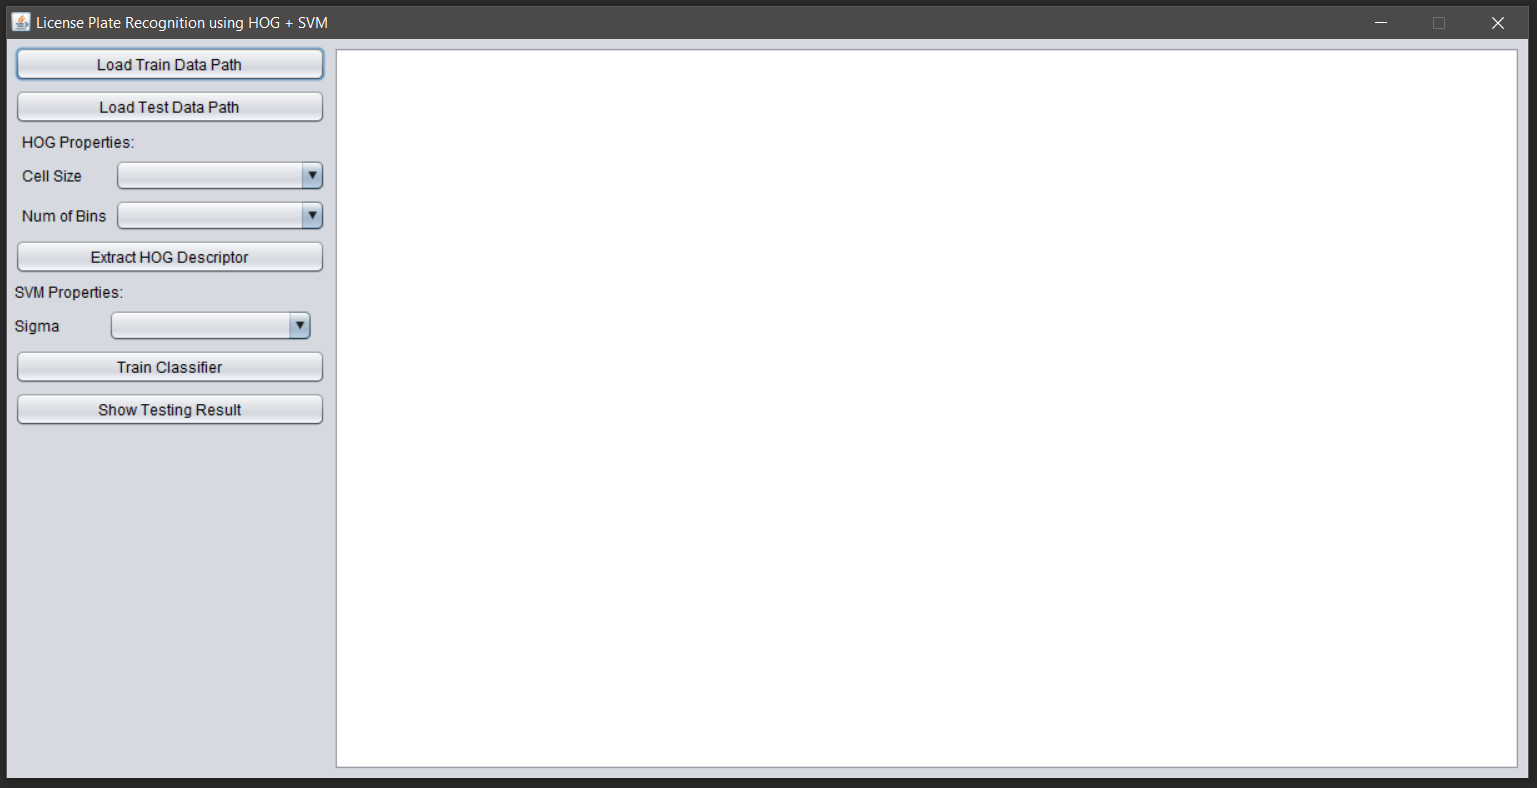
\includegraphics[width=16cm]{images/TampilanAntarmuka.png}
		\captionof{figure}{Tampilan antarmuka aplikasi pengenalan plat nomor kendaraan\\}
		\label{fig:TampilanAntarmuka}
	\end{minipage}
\end{adjustbox}\\
\\
\noindent Pada gambar \ref{fig:TampilanAntarmuka}, terdapat beberapa tombol diantaranya adalah tombol \textit{Load Train Data Path}, \textit{Load Test Data Path}, \textit{Extract HOG Descriptor}, \textit{Train Classifier}, dan \textit{Show Testing Result}. Terdapat juga beberapa tombol \textit{dropdown} yang berfungsi untuk memilih nilai dari parameter metode HOG dan SVM. Untuk metode HOG tombol \textit{dropdown} yang tersedia adalah tombol \textit{dropdown} untuk memilih ukuran sel (\textit{Cell Size}) dan jumlah \textit{bins} yang akan digunakan (\textit{Num of Bins}). Sedangkan untuk metode SVM tombol \textit{dropdown} yang tersedia adalah tombol \textit{dropdown} untuk memilih nilai sigma yang akan digunakan. Tahapan proses pengenalan plat nomor kendaraan di aplikasi terbagi menjadi dua, yaitu proses \textit{training} dan proses \textit{testing}. Tahapan proses \textit{training} pada aplikasi adalah sebagai berikut:
\begin{enumerate}
\item Memasukkan \textit{path} dari kumpulan citra yang akan digunakan sebagai data latih untuk proses pengenalan karakter.
\item Memasukkan ukuran sel dan jumlah \textit{bin} yang digunakan untuk metode HOG dengan memilih menggunakan tombol \textit{dropdown Cell Size} dan tombol \textit{dropdown Num of Bins}.
\item Klik tombol \textit{Extract HOG Descriptor} untuk menjalankan proses ekstraksi fitur.
\item Klik tombol \textit{Train Classifier} untuk menjalankan proses \textit{training}.
\end{enumerate}
\begin{adjustbox}{width=1\textwidth}
	\noindent\begin{minipage}{\linewidth}
		\centering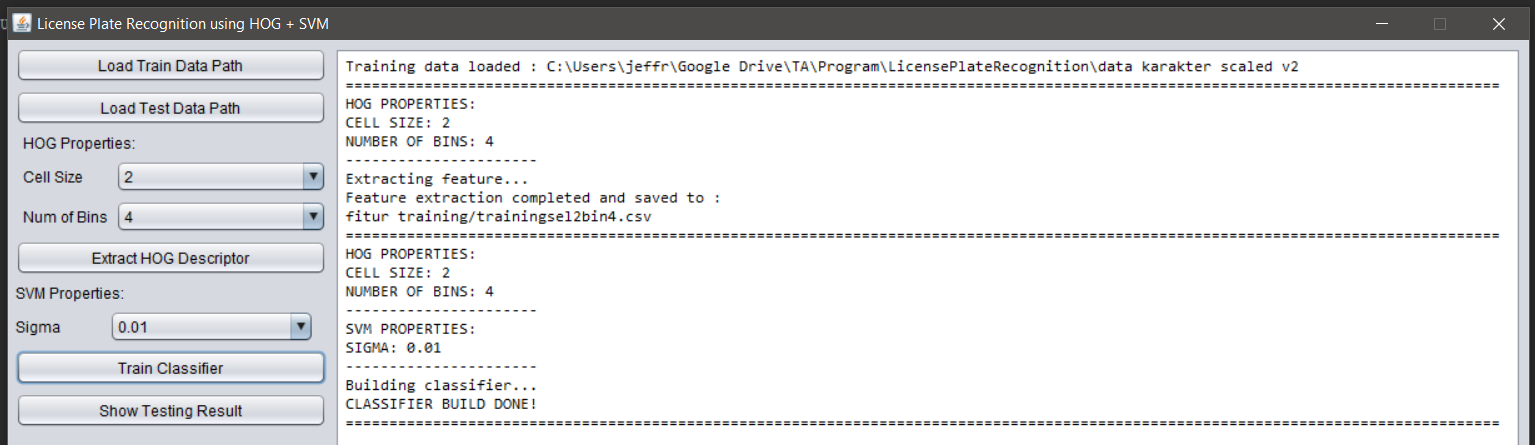
\includegraphics[width=16cm]{images/TampilanAntarmukaTraining.png}
		\captionof{figure}{Tampilan antarmuka hasil \textit{training}\\}
		\label{fig:TampilanAntarmukaTraining}
	\end{minipage}
\end{adjustbox}\\
\\
\noindent Pada gambar \ref{fig:TampilanAntarmukaTraining} aplikasi akan menampilkan \textit{path} dari folder citra yang akan digunakan sebagai data latih, ukuran sel dan jumlah \textit{bins} yang digunakan untuk metode HOG, pesan bahwa proses ekstraksi fitur sudah berjalan dan lokasi penyimpanan fitur, dan pesan bahwa proses \textit{training} sudah selesai.
\noindent Sedangkan untuk tahapan proses \textit{testing} pada aplikasi adalah sebagai berikut:
\begin{enumerate}
\item Lakukan proses \textit{training} terlebih dahulu.
\item Setelah proses \textit{training} selesai dilakukan, kemudian masukkan \textit{path} dari folder citra yang akan digunakan sebagai data uji.
\item Klik tombol \textit{Show Testing Result} untuk menjalankan proses testing otomatis.
\end{enumerate}
\begin{adjustbox}{width=1\textwidth}
	\noindent\begin{minipage}{\linewidth}
		\centering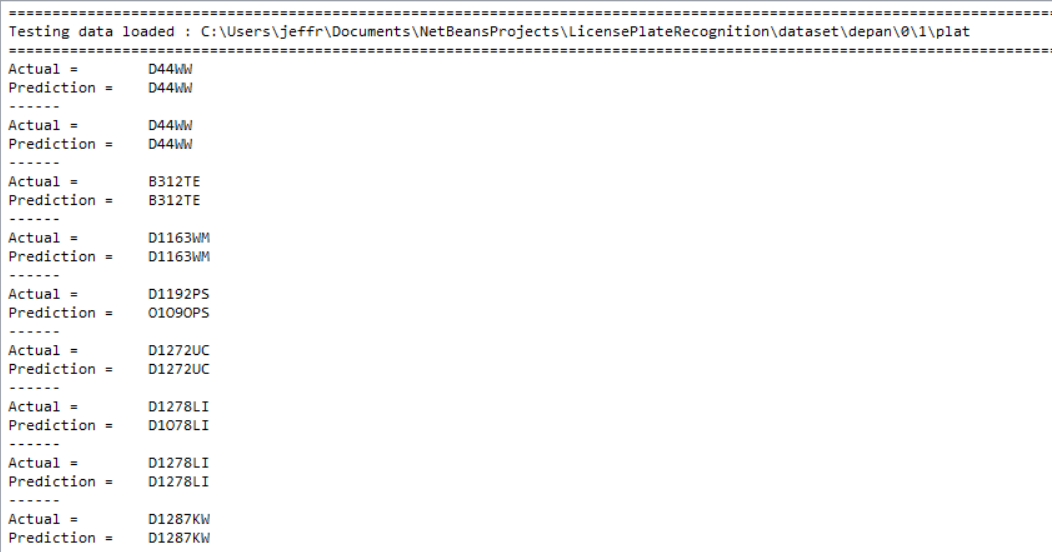
\includegraphics[width=16cm]{images/TampilanAntarmukaTesting1.png}
		\label{fig:TampilanAntarmukaTesting1}
	\end{minipage}
\end{adjustbox}\\
\begin{adjustbox}{width=1\textwidth}
	\noindent\begin{minipage}{\linewidth}
		\centering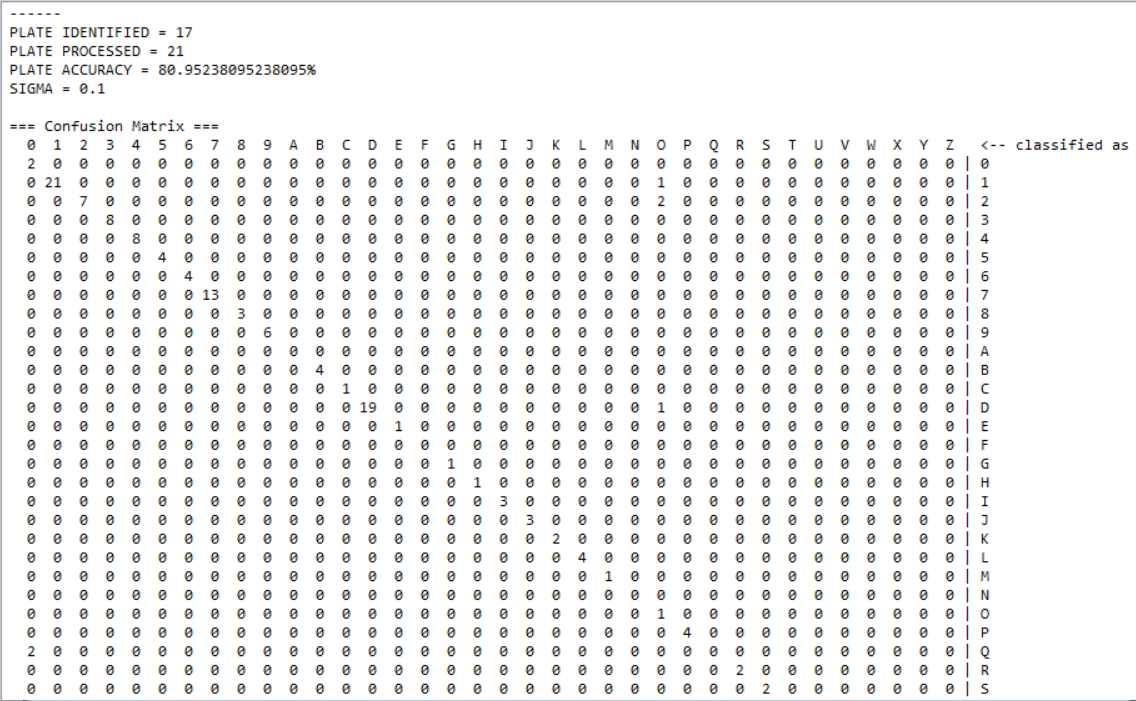
\includegraphics[width=16cm]{images/TampilanAntarmukaTesting2.png}
		\label{fig:TampilanAntarmukaTesting2}
	\end{minipage}
\end{adjustbox}\\
\begin{adjustbox}{width=1\textwidth}
	\noindent\begin{minipage}{\linewidth}
		\centering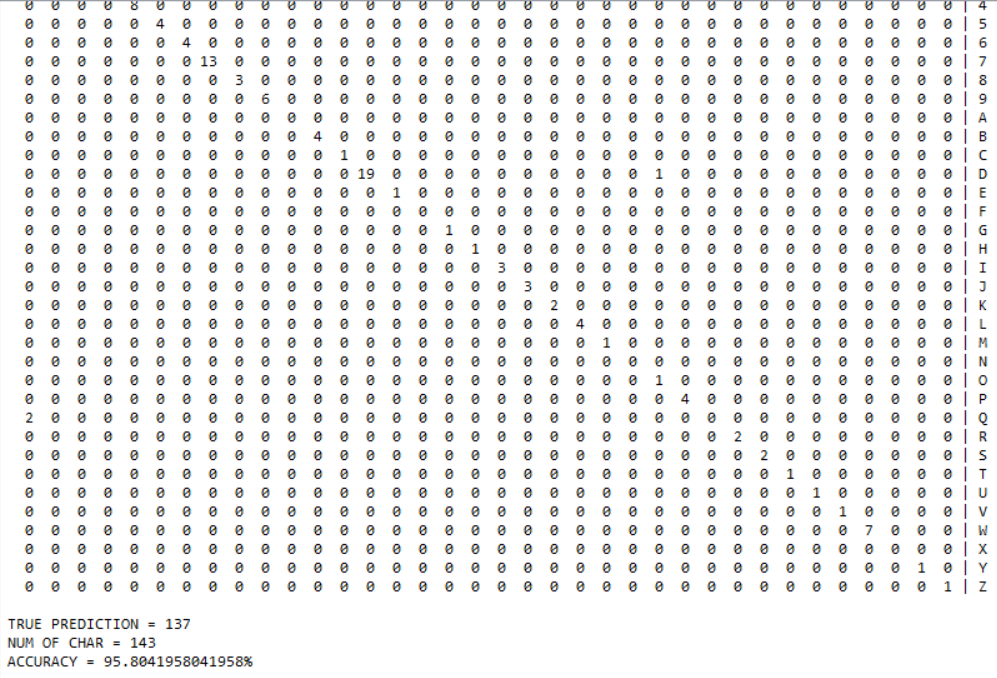
\includegraphics[width=16cm]{images/TampilanAntarmukaTesting3.png}
		\captionof{figure}{Tampilan antarmuka hasil \textit{testing} (Atas, tengah, bawah)\\}
		\label{fig:TampilanAntarmukaTesting3}
	\end{minipage}
\end{adjustbox}\\
\\
\noindent Pada gambar \ref{fig:TampilanAntarmukaTesting3} aplikasi akan menampilkan \textit{path} dari folder citra yang akan digunakan sebagai data uji, teks asli dari plat nomor pada citra beserta hasil prediksi dari SVM, jumlah plat yang teridentifikasi dengan benar, jumlah total plat yang diproses, akurasi plat yang terdeteksi dan teridentifikasi dengan benar, hasil dari \textit{confusion matrix} untuk klasifikasi karakter, jumlah karakter yang terklasifikasi dengan benar, jumlah keseluruhan karakter, dan akurasi dari klasifikasi karakter.\\
%Package cnn
%\subsubsection{Daftar \textit{Class} dan \textit{Method}}
%\noindent \textit{Class} CNN merupakan kelas yang berfungsi untuk melaksanakan proses \textit{Convolutional Neural Network} dengan arsitektur lapisan dan \textit{hyperparameter} yang telah ditentukan, lihat tabel \ref{tbl:classCNN}.
%\begingroup
%\setlength{\LTleft}{-20cm plus -1fill}
%\setlength{\LTright}{\LTleft}
%\begin{small}
%\begin{longtable}{|p{0.4cm}|p{2cm}|p{1.8cm}|p{1.8cm}|p{1.7cm}|p{3.55cm}|}
%	\caption{Daftar \textit{Method} pada \textit{Class} CNN \label{tbl:classCNN}}\\
%	\hline
%	\multirow{2}{*}{\textbf{No}} & \multirow{2}{*}{\textit{\textbf{Method}}} & \multicolumn{2}{c|}{\textit{\textbf{Input}}} & \multirow{2}{*}{\textit{\textbf{Output}}} & 
%	\multirow{2}{*}{\textbf{Keterangan}}\\
%	\cline{3-4}
%	& & \textbf{Tipe} & \textbf{Variabel} & & \\
%	\endfirsthead
%	\multicolumn{6}{c}{\textbf{\tablename~\thetable} Daftar \textit{Method} pada \textit{Class} CNN (Lanjutan)} \\ \hline
%	\multirow{2}{*}{\textbf{No}} & \multirow{2}{*}{\textit{\textbf{Method}}} & \multicolumn{2}{c|}{\textit{\textbf{Input}}} & \multirow{2}{*}{\textit{\textbf{Output}}} & 
%	\multirow{2}{*}{\textbf{Keterangan}}\\
%	\cline{3-4}
%	& & \textbf{Tipe} & \textbf{Variabel} & & \\
%	\endhead
%	\hline
%	1 & CNN & List$<$\newline Layer$>$,\newline double,\newline double,\newline int,\newline String & layers,\newline alpha,\newline alphaDivider,\newline saveModel,\newline pathModel & - & Konstruktor yang menerima dan menyimpan nilai \textit{hyperparameter} serta melakukan inisialisasi nilai pada kelas CNN.\\
%	\hline
%	2 & train & List$<$\newline TrainImage\newline$>$,\newline int & trainImg,\newline epoch & - & Melakukan tahap pembelajaran dari citra dengan pengulangan sebanyak \textit{epoch} serta menyimpan hasil pembelajaran.\\
%	\hline
%	3 & train & TrainImage & trainImg & - & Melakukan tahap pembelajaran untuk 1 citra, tahap \textit{forward} dan \textit{backward} yang mencakup menghitung turunan atau gradien lalu memperbarui nilai parameter berdasarkan gradien masing-masing.\\
%	\hline
%	4 & forward & TrainImage,\newline Process & img,\newline process & - & Melakukan tahap \textit{forward} pada setiap lapisan dan menghitung hasil berdasarkan proses pelatihan atau pengujian.\\
%	\hline
%	5 &  setGradient & TrainImage & img & - & Melakukan perhitungan gradien pada setiap lapisan.\\
%	\hline
%	6 & getData & - & - & List$<Data>$ & Menambahkan seluruh data yang telah dihitung pada setiap lapisan pada sebuah kelas \textit{List}.\\
%	\hline
%	7 & updateParams & - & - & - & Memperbarui parameter bobot berdasarkan data yang telah didapatkan dalam bentuk \textit{List}.\\
%	\hline
%	8 & update & int,\newline double,\newline double[] & j,\newline gradient,\newline weight & - & Menambahkan nilai bobot sesuai dengan gradiennya.\\
%	\hline
%	9 & test & List$<$\newline TrainImage\newline $>$ & trainImg & double & Melakukan tahap \textit{forward} untuk setiap gambar dan mengembalikan nilai akurasi.\\
%	\hline
%	10 & isHuman & double[][],\newline double & img,\newline threshold & boolean & Menguji adanya citra manusia yang dibatasi dengan probabilitas hasil pengujian.\\
%	\hline
%\end{longtable}
%\end{small}
%\endgroup

%\subsubsection{\textit{Class} CNNLoader}
%\noindent \textit{Class} CNNLoader merupakan kelas yang berfungsi untuk melakukan penyimpanan serta pemuatan model hasil pembelajaran \textit{Convolutional Neural Network}, lihat tabel \ref{tbl:classCNNLoader}.
%\begingroup
%\setlength{\LTleft}{-20cm plus -1fill}
%\setlength{\LTright}{\LTleft}
%\begin{small}
%\begin{longtable}{|p{0.4cm}|p{2cm}|p{1.8cm}|p{1.8cm}|p{1.7cm}|p{3.55cm}|}
%	\caption{Daftar \textit{Method} pada \textit{Class} CNNLoader \label{tbl:classCNNLoader}}\\
%	\hline
%	\multirow{2}{*}{\textbf{No}} & \multirow{2}{*}{\textit{\textbf{Method}}} & \multicolumn{2}{c|}{\textit{\textbf{Input}}} & \multirow{2}{*}{\textit{\textbf{Output}}} & 
%	\multirow{2}{*}{\textbf{Keterangan}}\\
%	\cline{3-4}
%	& & \textbf{Tipe} & \textbf{Variabel} & & \\
%	\endfirsthead
%	\multicolumn{6}{c}{\textbf{\tablename~\thetable} Daftar \textit{Method} pada \textit{Class} CNNLoader (Lanjutan)} \\
%	\hline
%	\multirow{2}{*}{\textbf{No}} & \multirow{2}{*}{\textit{\textbf{Method}}} & \multicolumn{2}{c|}{\textit{\textbf{Input}}} & \multirow{2}{*}{\textit{\textbf{Output}}} & 
%	\multirow{2}{*}{\textbf{Keterangan}}\\
%	\cline{3-4}
%	& & \textbf{Tipe} & \textbf{Variabel} & & \\
%	\endhead
%	\hline
%	1 & saveModel & String,\newline CNN & fileName,\newline cnn & - & Menyimpan model \textit{Convolutional Neural Network} dengan nama yang telah ditentukan.\\
%	\hline
%	2 & loadModel & String & fileName & CNN & Memuat model \textit{Convolutional Neural Network} yang telah disimpan sebelumnya.\\
%	\hline
%\end{longtable}
%\end{small}
%\endgroup

%Package cnn.layer
%\subsubsection{\textit{Class} Data}
%\noindent \textit{Class} Data merupakan kelas yang berfungsi untuk menyimpan data yang digunakan pada tahap \textit{Convolutional Neural Network}, lihat tabel \ref{tbl:classData}.
%\begingroup
%\setlength{\LTleft}{-20cm plus -1fill}
%\setlength{\LTright}{\LTleft}
%\begin{small}
%\begin{longtable}{|p{0.4cm}|p{2cm}|p{1.8cm}|p{1.8cm}|p{1.7cm}|p{3.55cm}|}
%	\caption{Daftar \textit{Method} pada \textit{Class} Data \label{tbl:classData}}\\
%	\hline
%	\multirow{2}{*}{\textbf{No}} & \multirow{2}{*}{\textit{\textbf{Method}}} & \multicolumn{2}{c|}{\textit{\textbf{Input}}} & \multirow{2}{*}{\textit{\textbf{Output}}} & 
%	\multirow{2}{*}{\textbf{Keterangan}}\\
%	\cline{3-4}
%	& & \textbf{Tipe} & \textbf{Variabel} & & \\
%	\endfirsthead
%	\multicolumn{6}{c}{\textbf{\tablename~\thetable} Daftar \textit{Method} pada \textit{Class} Data (Lanjutan)} \\
%	\hline
%	\multirow{2}{*}{\textbf{No}} & \multirow{2}{*}{\textit{\textbf{Method}}} & \multicolumn{2}{c|}{\textit{\textbf{Input}}} & \multirow{2}{*}{\textit{\textbf{Output}}} & 
%	\multirow{2}{*}{\textbf{Keterangan}}\\
%	\cline{3-4}
%	& & \textbf{Tipe} & \textbf{Variabel} & & \\
%	\endhead
%	\hline
%	1 & Data & Size & size & - & Konstruktor yang menerima dan menyimpan besar ukuran.\\
%	\hline
%	2 & addImage-\newline Data & double[][] & trainImg & - & Menyimpan nilai dari citra.\\
%	\hline
%	3 & getSize & - & - & Size & Digunakan untuk mendapatkan ukuran dari data.\\
%	\hline
%	4 & getWeight & int & index & double & Digunakan untuk mendapatkan bobot pada indeks 1 dimensi.\\
%	\hline
%	5 & getWeight & int,\newline int,\newline int & x,\newline y,\newline depth & double & Digunakan untuk mendapatkan bobot pada indeks 3 dimensi.\\
%	\hline
%	6 & setWeight & double & value & - & Digunakan untuk mendapatkan bobot pada indeks 1 dimensi.\\
%	\hline
%	7 & setWeight & int,\newline int,\newline int,\newline double & x,\newline y,\newline depth,\newline value & - & Digunakan untuk menetapkan nilai bobot pada indeks 3 dimensi.\\
%	\hline
%	8 & addWeight & int,\newline int,\newline int,\newline double & x,\newline y,\newline depth,\newline value & - & Digunakan untuk menambahkan nilai bobot.\\
%	\hline
%	9 & getGradient & int,\newline int,\newline int & x,\newline y,\newline depth & double & Digunakan untuk mendapatkan ukuran dari data pada indeks 3 dimensi.\\
%	\hline
%	10 & getGradient & int & index & double & Digunakan untuk mendapatkan ukuran dari data pada indeks 1 dimensi\\
%	\hline
%	11 & setGradient & int,\newline int,\newline int,\newline double & x,\newline y,\newline depth,\newline value & - & Digunakan untuk menentukan nilai gradien pada indeks 3 dimensi.\\
%	\hline
%	12 & setGradient & int & value & - & Digunakan untuk menentukan nilai gradien pada indeks 1 dimensi.\\
%	\hline
%	13 & addGradient & int,\newline int,\newline int,\newline double & x,\newline y,\newline depth,\newline value & - & Digunakan untuk nambahkan nilai gradien dengan indeks 3 dimensi.\\
%	\hline
%	14 & addGradient & int,\newline double & index,\newline value & - & Digunakan untuk nambahkan nilai gradien pada indeks 1 dimensi.\\
%	\hline
%	15 & calculate-\newline Index & int,\newline int,\newline int & x,\newline y,\newline depth & int & Digunakan untuk mendapatkan indeks pada 1 dimensi.\\
%	\hline
%	16 & clearGradient & - & - & - & Digunakan untuk hapus seluruh gradien.\\
%	\hline
%	17 & getWeights & - & - & double[] & Digunakan untuk mendapatkan seluruh bobot.\\
%	\hline
%	18 & getGradients & - & - & double[] & Digunakan untuk mendapatkan seluruh gradien.\\
%	\hline
%\end{longtable}
%\end{small}
%\endgroup

%\subsubsection{\textit{Class} Size}
%\noindent \textit{Class} Size merupakan kelas yang berfungsi untuk menyimpan informasi ukuran lebar, tinggi, dan kedalaman. Penjelasan mengenai kelas ini dapat dilihat pada tabel \ref{tbl:classSize}.
%\begingroup
%\setlength{\LTleft}{-20cm plus -1fill}
%\setlength{\LTright}{\LTleft}
%\begin{small}
%\begin{longtable}{|p{0.4cm}|p{2cm}|p{1.8cm}|p{1.8cm}|p{1.7cm}|p{3.55cm}|}
%	\caption{Daftar \textit{Method} pada \textit{Class} Size \label{tbl:classSize}}\\
%	\hline
%	\multirow{2}{*}{\textbf{No}} & \multirow{2}{*}{\textit{\textbf{Method}}} & \multicolumn{2}{c|}{\textit{\textbf{Input}}} & \multirow{2}{*}{\textit{\textbf{Output}}} & 
%	\multirow{2}{*}{\textbf{Keterangan}}\\
%	\cline{3-4}
%	& & \textbf{Tipe} & \textbf{Variabel} & & \\
%	\endfirsthead
%	\multicolumn{6}{c}{\textbf{\tablename~\thetable} Daftar \textit{Method} pada \textit{Class} Size (Lanjutan)} \\
%	\hline
%	\multirow{2}{*}{\textbf{No}} & \multirow{2}{*}{\textit{\textbf{Method}}} & \multicolumn{2}{c|}{\textit{\textbf{Input}}} & \multirow{2}{*}{\textit{\textbf{Output}}} & 
%	\multirow{2}{*}{\textbf{Keterangan}}\\
%	\cline{3-4}
%	& & \textbf{Tipe} & \textbf{Variabel} & & \\
%	\endhead
%	\hline
%	1 & Size & - & - & - & Konstruktor kosong ketika objek dibuat tanpa parameter.\\
%	\hline
%	2 & Size & int,\newline int,\newline int & width,\newline height,\newline depth & - & Konstruktor yang menerima dan menerima informasi ukuran.\\
%	\hline
%	3 & getWidth & - & - & int & Digunakan untuk mendapatkan lebar citra.\\
%	\hline
%	2 & setWidth & int & width & - & Digunakan untuk menentukan lebar citra.\\
%	\hline
%	2 & getHeight & - & - & int & Digunakan untuk mendapatkan tinggi citra.\\
%	\hline
%	2 & setHeight & int & height & - & Digunakan untuk menentukan tinggi citra.\\
%	\hline
%	2 & getDepth & - & - & int & Digunakan untuk mendapatkan kedalaman citra.\\
%	\hline
%	2 & setDepth & int & depth & - & Digunakan untuk menentukan kedalaman citra.\\
%	\hline
%	2 & toString & - & - & String & Mengembalikan informasi ukuran dalam bentuk text.\\
%	\hline
%\end{longtable}
%\end{small}
%\endgroup

%Package cnn.layer
%\subsubsection{\textit{Class} Layer}
%\noindent \textit{Class} Layer merupakan sebuah kelas abstrak untuk lapisan pada \textit{Convolutional Neural Network}. Penjelasan mengenai kelas ini dapat dilihat pada tabel \ref{tbl:classLayer}.
%\begingroup
%\setlength{\LTleft}{-20cm plus -1fill}
%\setlength{\LTright}{\LTleft}
%\begin{small}
%\begin{longtable}{|p{0.4cm}|p{2cm}|p{1.8cm}|p{1.8cm}|p{1.7cm}|p{3.55cm}|}
%	\caption{Daftar \textit{Method} pada \textit{Class} Layer \label{tbl:classLayer}}\\
%	\hline
%	\multirow{2}{*}{\textbf{No}} & \multirow{2}{*}{\textit{\textbf{Method}}} & \multicolumn{2}{c|}{\textit{\textbf{Input}}} & \multirow{2}{*}{\textit{\textbf{Output}}} & 
%	\multirow{2}{*}{\textbf{Keterangan}}\\
%	\cline{3-4}
%	& & \textbf{Tipe} & \textbf{Variabel} & & \\
%	\endfirsthead
%	\multicolumn{6}{c}{\textbf{\tablename~\thetable} Daftar \textit{Method} pada \textit{Class} Layer (Lanjutan)} \\
%	\hline
%	\multirow{2}{*}{\textbf{No}} & \multirow{2}{*}{\textit{\textbf{Method}}} & \multicolumn{2}{c|}{\textit{\textbf{Input}}} & \multirow{2}{*}{\textit{\textbf{Output}}} & 
%	\multirow{2}{*}{\textbf{Keterangan}}\\
%	\cline{3-4}
%	& & \textbf{Tipe} & \textbf{Variabel} & & \\
%	\endhead
%	\hline
%	1 & forward & Data & inData & Data & Menerima data masukan untuk diproses dan menghasilkan data keluaran.\\
%	\hline
%	2 & setGradient & - & - & - & Menghitung dan menentukan nilai gradien.\\
%	\hline
%	3 & getData & - & - & List$<$Data$>$ & Digunakan untuk mendapatkan seluruh data dalam bentuk \textit{List}.\\
%	\hline
%	4 & getType & - & - & LayerType & Digunakan untuk mendapatkan keterangan jenis lapisan.\\
%	\hline
%	5 & setType & LayerType & type & - & Digunakan untuk menentukan jenis dari lapisan.\\
%	\hline
%	6 & getMapSize & - & - & Size & Digunakan untuk mendapatkan informasi ukuran.\\
%	\hline
%	7 & setMapSize & Size & mapSize & - & Digunakan untuk menentukan ukuran.\\
%	\hline
%	8 & setInData & Data & data & - & Digunakan untuk menentukan data masukan.\\
%	\hline
%	9 & getOutData & - & - & Data & Digunakan untuk mendapatkan data keluaran.\\
%	\hline
%	10 & setData & Data & data & - & Digunakan untuk menentukan data keluaran.\\
%	\hline
%\end{longtable}
%\end{small}
%\endgroup

%\subsubsection{\textit{Class} InputLayer}
%\noindent \textit{Class} InputLayer merupakan kelas untuk menyimpan informasi pada lapisan masukan dan di-\textit{extends} dengan \textit{class} Layer. Penjelasan kelas ini dapat dilihat pada tabel \ref{tbl:classInputLayer}.
%\begingroup
%\setlength{\LTleft}{-20cm plus -1fill}
%\setlength{\LTright}{\LTleft}
%\begin{small}
%\begin{longtable}{|p{0.4cm}|p{2cm}|p{1.8cm}|p{1.8cm}|p{1.7cm}|p{3.55cm}|}
%	\caption{Daftar \textit{Method} pada \textit{Class} InputLayer \label{tbl:classInputLayer}}\\
%	\hline
%	\multirow{2}{*}{\textbf{No}} & \multirow{2}{*}{\textit{\textbf{Method}}} & \multicolumn{2}{c|}{\textit{\textbf{Input}}} & \multirow{2}{*}{\textit{\textbf{Output}}} & 
%	\multirow{2}{*}{\textbf{Keterangan}}\\
%	\cline{3-4}
%	& & \textbf{Tipe} & \textbf{Variabel} & & \\
%	\endfirsthead
%	\multicolumn{6}{c}{\textbf{\tablename~\thetable} Daftar \textit{Method} pada \textit{Class} InputLayer (Lanjutan)} \\
%	\hline
%	\multirow{2}{*}{\textbf{No}} & \multirow{2}{*}{\textit{\textbf{Method}}} & \multicolumn{2}{c|}{\textit{\textbf{Input}}} & \multirow{2}{*}{\textit{\textbf{Output}}} & 
%	\multirow{2}{*}{\textbf{Keterangan}}\\
%	\cline{3-4}
%	& & \textbf{Tipe} & \textbf{Variabel} & & \\
%	\endhead
%	\hline
%	1 & InputLayer & Size & mapSize & - & Konstruktor untuk menerima parameter dan menentukan jenis layer.\\
%	\hline
%	2 & setTrain-\newline Image & TrainImage & trainImg & - & Digunakan untuk menentukan citra masukan yang akan diproses.\\
%	\hline
%	3 & getImgInput & - & - & double[][] & Digunakan untuk mendapatkan informasi mengenai citra masukan.\\
%	\hline
%	4 & getLabel & - & - & int & Digunakan untuk mendapatkan label dari citra masukan.\\
%	\hline
%	5 & forward & Data & data & Data & Untuk menerima data masukan dan menentukan data keluaran serta mengembalikan nilai keluaran tersebut.\\
%	\hline
%	6 & setGradient & - & - & - & Pada lapisan masukan tidak dilakukan perhitungan gradien.\\
%	\hline
%	7 & getData & - & - & List$<$Data$>$ & Mengembalikan list kosong karena tidak terdapat data yang perlu diperbarui.\\
%	\hline
%\end{longtable}
%\end{small}
%\endgroup

%\subsubsection{\textit{Class} ConvolutionLayer}
%\noindent \textit{Class} ConvolutionLayer merupakan kelas untuk proses konvolusi pada tahap \textit{forward} maupun \textit{backward} dan di-\textit{extends} dengan \textit{class} Layer. Penjelasan kelas ini dapat dilihat pada tabel \ref{tbl:classConvolutionLayer}.
%\begingroup
%\setlength{\LTleft}{-20cm plus -1fill}
%\setlength{\LTright}{\LTleft}
%\begin{small}
%\begin{longtable}{|p{0.4cm}|p{2cm}|p{1.8cm}|p{1.8cm}|p{1.7cm}|p{3.55cm}|}
%	\caption{Daftar \textit{Method} pada \textit{Class} ConvolutionLayer \label{tbl:classConvolutionLayer}}\\
%	\hline
%	\multirow{2}{*}{\textbf{No}} & \multirow{2}{*}{\textit{\textbf{Method}}} & \multicolumn{2}{c|}{\textit{\textbf{Input}}} & \multirow{2}{*}{\textit{\textbf{Output}}} & 
%	\multirow{2}{*}{\textbf{Keterangan}}\\
%	\cline{3-4}
%	& & \textbf{Tipe} & \textbf{Variabel} & & \\
%	\endfirsthead
%	\multicolumn{6}{c}{\textbf{\tablename~\thetable} Daftar \textit{Method} pada \textit{Class} ConvolutionLayer (Lanjutan)} \\
%	\hline
%	\multirow{2}{*}{\textbf{No}} & \multirow{2}{*}{\textit{\textbf{Method}}} & \multicolumn{2}{c|}{\textit{\textbf{Input}}} & \multirow{2}{*}{\textit{\textbf{Output}}} & 
%	\multirow{2}{*}{\textbf{Keterangan}}\\
%	\cline{3-4}
%	& & \textbf{Tipe} & \textbf{Variabel} & & \\
%	\endhead
%	\hline
%	1 & Convolution-\newline Layer & Size & kernelSize & - & Konstruktor yang menerima ukuran \textit{kernel} dan melakukan inisialisasi atribut.\\
%	\hline
%	2 & initOutData & Data & inData & Data & Melakukan inisialisasi ukuran untuk data keluaran.\\
%	\hline
%	3 & forward & Data & inData & Data & Melakukan proses perhitungan konvolusi data masukan dengan \textit{kernel} dan bias, lalu hasilnya disimpan dan dikembalikan sebagai data keluaran untuk diproses pada lapisan selanjutnya.\\
%	\hline
%	4 & setGradient & - & - & - & Menghitung gradien pada lapisan konvolusi dengan menggunakan gradien dari lapisan selanjutnya.\\
%	\hline
%	5 & getData & - & - & List$<$Data$>$ & Mengembalikan seluruh data \textit{kernel} dan bias yang digunakan pada lapisan konvolusi.\\
%	\hline
%\end{longtable}
%\end{small}
%\endgroup

%\subsubsection{\textit{Class} RELULayer}
%\noindent \textit{Class} RELU merupakan kelas yang di-\textit{extends} dengan \textit{class} Layer untuk menghitung hasil data masukan yang dimasukkan ke fungsi aktivasi \textit{rectified linear unit} (ReLU). Penjelasan kelas ini dapat dilihat pada tabel \ref{tbl:classRELULayer}.
%\begingroup
%\setlength{\LTleft}{-20cm plus -1fill}
%\setlength{\LTright}{\LTleft}
%\begin{small}
%\begin{longtable}{|p{0.4cm}|p{2cm}|p{1.8cm}|p{1.8cm}|p{1.7cm}|p{3.55cm}|}
%	\caption{Daftar \textit{Method} pada \textit{Class} RELULayer \label{tbl:classRELULayer}}\\
%	\hline
%	\multirow{2}{*}{\textbf{No}} & \multirow{2}{*}{\textit{\textbf{Method}}} & \multicolumn{2}{c|}{\textit{\textbf{Input}}} & \multirow{2}{*}{\textit{\textbf{Output}}} & 
%	\multirow{2}{*}{\textbf{Keterangan}}\\
%	\cline{3-4}
%	& & \textbf{Tipe} & \textbf{Variabel} & & \\
%	\endfirsthead
%	\multicolumn{6}{c}{\textbf{\tablename~\thetable} Daftar \textit{Method} pada \textit{Class} RELULayer (Lanjutan)} \\
%	\hline
%	\multirow{2}{*}{\textbf{No}} & \multirow{2}{*}{\textit{\textbf{Method}}} & \multicolumn{2}{c|}{\textit{\textbf{Input}}} & \multirow{2}{*}{\textit{\textbf{Output}}} & 
%	\multirow{2}{*}{\textbf{Keterangan}}\\
%	\cline{3-4}
%	& & \textbf{Tipe} & \textbf{Variabel} & & \\
%	\endhead
%	\hline
%	1 & reluActivation & double & value & double & Menghitung sebuah nilai untuk digunakan pada fungsi aktivasi ReLU.\\
%	\hline
%	2 & forward & Data & inData & Data & Menghitung seluruh nilai dari data masukan dengan fungsi aktivasi ReLU.\\
%	\hline
%	3 & setGradient & - & - & - & Menghitung gradien dengan turunan dari fungsi aktivasi ReLU.\\
%	\hline
%	4 & getData & - & - & List$<$Data$>$ & Mengembalikan list data kosong karena tidak terdapat data yang perlu diperbarui.\\
%	\hline
%\end{longtable}
%\end{small}
%\endgroup

%\subsubsection{\textit{Class} SubsamplingLayer}
%\noindent \textit{Class} SubsamplingLayer merupakan kelas untuk menyimpan hasil dari proses \textit{subsampling} atau \textit{pooling} dan di-\textit{extends} dengan \textit{class} Layer. Penjelasan kelas ini dapat dilihat pada tabel \ref{tbl:classSubsamplingLayer}.
%\begingroup
%\setlength{\LTleft}{-20cm plus -1fill}
%\setlength{\LTright}{\LTleft}
%\begin{small}
%\begin{longtable}{|p{0.4cm}|p{2cm}|p{1.8cm}|p{1.8cm}|p{1.7cm}|p{3.55cm}|}
%	\caption{Daftar \textit{Method} pada \textit{Class} SubsamplingLayer \label{tbl:classSubsamplingLayer}}\\
%	\hline
%	\multirow{2}{*}{\textbf{No}} & \multirow{2}{*}{\textit{\textbf{Method}}} & \multicolumn{2}{c|}{\textit{\textbf{Input}}} & \multirow{2}{*}{\textit{\textbf{Output}}} & 
%	\multirow{2}{*}{\textbf{Keterangan}}\\
%	\cline{3-4}
%	& & \textbf{Tipe} & \textbf{Variabel} & & \\
%	\endfirsthead
%	\multicolumn{6}{c}{\textbf{\tablename~\thetable} Daftar \textit{Method} pada \textit{Class} SubsamplingLayer (Lanjutan)} \\
%	\hline
%	\multirow{2}{*}{\textbf{No}} & \multirow{2}{*}{\textit{\textbf{Method}}} & \multicolumn{2}{c|}{\textit{\textbf{Input}}} & \multirow{2}{*}{\textit{\textbf{Output}}} & 
%	\multirow{2}{*}{\textbf{Keterangan}}\\
%	\cline{3-4}
%	& & \textbf{Tipe} & \textbf{Variabel} & & \\
%	\endhead
%	\hline
%	1 & Sub-\newline sampling-\newline Layer & Size & scaleSize & - & Konstruktor yang menerima ukuran untuk \textit{pooling}.\\
%	\hline
%	2 & initOutData & Data & inData & Data & Melakukan inisialisasi ukuran untuk data keluaran.\\
%	\hline
%	3 & initMaxData & Data & outData & Data & Melakukan inisialisasi ukuran untuk indeks dengan nilai tertinggi.\\
%	\hline
%	2 & forward & Data & inData & Data & Melakukan proses \textit{pooling} sesuai dengan ukuran yang telah ditentukan dan menyimpan indeks dari nilai yang tertinggi untuk digunakan saat tahap \textit{backward}.\\
%	\hline
%	3 & setGradient & - & - & - & Menentukan nilai gradien berdasarkan nilai tertinggi saat tahap \textit{forward} dan nilai lainnya adalah 0.\\
%	\hline
%	4 & getData & - & - & List$<$Data$>$ & Mengembalikan list data kosong karena tidak terdapat data yang perlu diperbarui.\\
%	\hline
%\end{longtable}
%\end{small}
%\endgroup

%\subsubsection{\textit{Class} FullyConnectedLayer}
%\noindent \textit{Class} FullyConnectedLayer merupakan kelas yang berfungsi untuk menerima seluruh data hasil dari lapisan sebelumnya dan selanjutnya dimasukkan ke fungsi. \textit{Class} ini juga di-\textit{extends} dengan \textit{class} Layer. Penjelasan kelas ini dapat dilihat pada tabel \ref{tbl:classFullyConnectedLayer}.
%\begingroup
%\setlength{\LTleft}{-20cm plus -1fill}
%\setlength{\LTright}{\LTleft}
%\begin{small}
%\begin{longtable}{|p{0.4cm}|p{2cm}|p{1.8cm}|p{1.8cm}|p{1.7cm}|p{3.55cm}|}
%	\caption{Daftar \textit{Method} pada \textit{Class} FullyConnectedLayer \label{tbl:classFullyConnectedLayer}}\\
%	\hline
%	\multirow{2}{*}{\textbf{No}} & \multirow{2}{*}{\textit{\textbf{Method}}} & \multicolumn{2}{c|}{\textit{\textbf{Input}}} & \multirow{2}{*}{\textit{\textbf{Output}}} & 
%	\multirow{2}{*}{\textbf{Keterangan}}\\
%	\cline{3-4}
%	& & \textbf{Tipe} & \textbf{Variabel} & & \\
%	\endfirsthead
%	\multicolumn{6}{c}{\textbf{\tablename~\thetable} Daftar \textit{Method} pada \textit{Class} FullyConnectedLayer (Lanjutan)} \\
%	\hline
%	\multirow{2}{*}{\textbf{No}} & \multirow{2}{*}{\textit{\textbf{Method}}} & \multicolumn{2}{c|}{\textit{\textbf{Input}}} & \multirow{2}{*}{\textit{\textbf{Output}}} & 
%	\multirow{2}{*}{\textbf{Keterangan}}\\
%	\cline{3-4}
%	& & \textbf{Tipe} & \textbf{Variabel} & & \\
%	\endhead
%	\hline
%	1 & Fully-\newline Connected-\newline Layer & Size & kernelSize & - & Konstruktor yang menerima ukuran \textit{kernel} dan inisialisasi atribut.\\
%	\hline
%	2 & forward & Data & inData & Data & Membentuk data masukan dalam bentuk 1 dimensi dan dikalikan dengan \textit{kernel} yang berukuran sama dengan masukan, kemudian dijumlahkan sebagai data keluaran.\\
%	\hline
%	3 & setGradient & - & - & - & Menghitung dan menentukan nilai gradien pada data masukan, \textit{kernel}, serta bias.\\
%	\hline
%	4 & getData & - & - & List$<$Data$>$ & Mengembalikan seluruh data \textit{kernel} dan bias yang digunakan pada lapisan ini.\\
%	\hline
%\end{longtable}
%\end{small}
%\endgroup

%\subsubsection{\textit{Class} SoftmaxLayer}
%\noindent \textit{Class} SoftmaxLayer merupakan kelas yang di-\textit{extends} dengan \textit{class} Layer untuk menghitung hasil data masukan yang dimasukkan ke fungsi \textit{softmax}. Penjelasan kelas ini dapat dilihat pada tabel \ref{tbl:classSoftmaxLayer}.
%\begingroup
%\setlength{\LTleft}{-20cm plus -1fill}
%\setlength{\LTright}{\LTleft}
%\begin{small}
%\begin{longtable}{|p{0.4cm}|p{2cm}|p{1.8cm}|p{1.8cm}|p{1.7cm}|p{3.55cm}|}
%	\caption{Daftar \textit{Method} pada \textit{Class} SoftmaxLayer \label{tbl:classSoftmaxLayer}}\\
%	\hline
%	\multirow{2}{*}{\textbf{No}} & \multirow{2}{*}{\textit{\textbf{Method}}} & \multicolumn{2}{c|}{\textit{\textbf{Input}}} & \multirow{2}{*}{\textit{\textbf{Output}}} & 
%	\multirow{2}{*}{\textbf{Keterangan}}\\
%	\cline{3-4}
%	& & \textbf{Tipe} & \textbf{Variabel} & & \\
%	\endfirsthead
%	\multicolumn{6}{c}{\textbf{\tablename~\thetable} Daftar \textit{Method} pada \textit{Class} SoftmaxLayer (Lanjutan)} \\
%	\hline
%	\multirow{2}{*}{\textbf{No}} & \multirow{2}{*}{\textit{\textbf{Method}}} & \multicolumn{2}{c|}{\textit{\textbf{Input}}} & \multirow{2}{*}{\textit{\textbf{Output}}} & 
%	\multirow{2}{*}{\textbf{Keterangan}}\\
%	\cline{3-4}
%	& & \textbf{Tipe} & \textbf{Variabel} & & \\
%	\endhead
%	\hline
%	1 & Softmax-\newline Layer & Size & size & - & Konstruktor yang menerima ukuran hasil akhir dari \textit{Convolutional Neural Network}.\\
%	\hline
%	2 & forward & Data & inData & Data & Melakukan perhitungan menggunakan fungsi \textit{softmax} yang telah dinormalisasi dengan nilai maksimal nilai masukan.\\
%	\hline
%	3 & setGradient & - & - & - & Menghitung nilai \textit{error} dari label sebenarnya.\\
%	\hline
%	4 & getData & - & - & List$<$Data$>$ & Mengembalikan list data kosong karena tidak terdapat data yang perlu diperbarui.\\
%	\hline
%\end{longtable}
%\end{small}
%\endgroup

%Package kalman
%\subsubsection{\textit{Class} Kalman}
%\noindent \textit{Class} Kalman merupakan kelas yang berfungsi untuk melakukan proses Kalman \textit{filtering} yang mencakup tahap prediksi dan pembaruan, lihat tabel \ref{tbl:classKalman}.
%\begingroup
%\setlength{\LTleft}{-20cm plus -1fill}
%\setlength{\LTright}{\LTleft}
%\begin{small}
%\begin{longtable}{|p{0.4cm}|p{2cm}|p{1.8cm}|p{1.8cm}|p{1.7cm}|p{3.55cm}|}
%	\caption{Daftar \textit{Method} pada \textit{Class} Kalman \label{tbl:classKalman}}\\
%	\hline
%	\multirow{2}{*}{\textbf{No}} & \multirow{2}{*}{\textit{\textbf{Method}}} & \multicolumn{2}{c|}{\textit{\textbf{Input}}} & \multirow{2}{*}{\textit{\textbf{Output}}} & 
%	\multirow{2}{*}{\textbf{Keterangan}}\\
%	\cline{3-4}
%	& & \textbf{Tipe} & \textbf{Variabel} & & \\
%	\endfirsthead
%	\multicolumn{6}{c}{\textbf{\tablename~\thetable} Daftar \textit{Method} pada \textit{Class} Kalman (Lanjutan)} \\
%	\hline
%	\multirow{2}{*}{\textbf{No}} & \multirow{2}{*}{\textit{\textbf{Method}}} & \multicolumn{2}{c|}{\textit{\textbf{Input}}} & \multirow{2}{*}{\textit{\textbf{Output}}} & 
%	\multirow{2}{*}{\textbf{Keterangan}}\\
%	\cline{3-4}
%	& & \textbf{Tipe} & \textbf{Variabel} & & \\
%	\endhead
%	\hline
%	1 & Kalman & double & rk & - & Konstruktor yang menerima parameter dan melakukan inisialisasi atribut.\\
%	\hline
%	2 & predict & - & - & double & Menghitung dan mengembalikan hasil prediksi berdasarkan data sebelumnya.\\
%	\hline
%	3 & update & double & zk & - & Memperbarui nilai pada Kalman sesuai dengan kondisi sebenarnya.\\
%	\hline
%\end{longtable}
%\end{small}
%\endgroup

%\subsubsection{\textit{Class} KalmanPosition}
%\noindent \textit{Class} KalmanPosition merupakan kelas yang berisi posisi $x_{1}$, $y_{1}$, $x_{2}$, dan $y_{2}$ dengan tipe Kalman, lihat tabel \ref{tbl:classKalmanPosition}.
%\begingroup
%\setlength{\LTleft}{-20cm plus -1fill}
%\setlength{\LTright}{\LTleft}
%\begin{small}
%\begin{longtable}{|p{0.4cm}|p{2cm}|p{1.8cm}|p{1.8cm}|p{1.7cm}|p{3.55cm}|}
%	\caption{Daftar \textit{Method} pada \textit{Class} KalmanPosition \label{tbl:classKalmanPosition}}\\
%	\hline
%	\multirow{2}{*}{\textbf{No}} & \multirow{2}{*}{\textit{\textbf{Method}}} & \multicolumn{2}{c|}{\textit{\textbf{Input}}} & \multirow{2}{*}{\textit{\textbf{Output}}} & 
%	\multirow{2}{*}{\textbf{Keterangan}}\\
%	\cline{3-4}
%	& & \textbf{Tipe} & \textbf{Variabel} & & \\
%	\endfirsthead
%	\multicolumn{6}{c}{\textbf{\tablename~\thetable} Daftar \textit{Method} pada \textit{Class} KalmanPosition (Lanjutan)} \\
%	\hline
%	\multirow{2}{*}{\textbf{No}} & \multirow{2}{*}{\textit{\textbf{Method}}} & \multicolumn{2}{c|}{\textit{\textbf{Input}}} & \multirow{2}{*}{\textit{\textbf{Output}}} & 
%	\multirow{2}{*}{\textbf{Keterangan}}\\
%	\cline{3-4}
%	& & \textbf{Tipe} & \textbf{Variabel} & & \\
%	\endhead
%	\hline
%	1 & Kalman-\newline Position & double & rk & - & Konstruktor yang menerima parameter dan melakukan inisialisasi setiap posisi.\\
%	\hline
%	2 & getX1 & - & - & Kalman & Digunakan untuk mendapatkan posisi $x_{1}$.\\
%	\hline
%	3 & setX1 & Kalman & x1 & Kalman & Digunakan untuk menentukan $x_{1}$.\\
%	\hline
%	4 & getY1 & - & - & Kalman & Digunakan untuk mendapatkan posisi $y_{1}$.\\
%	\hline
%	5 & setY1 & Kalman & y1 & - & Digunakan untuk menentukan posisi $y_{1}$.\\
%	\hline
%	6 & getX2 & - & - & Kalman & Digunakan untuk mendapatkan posisi $x_{2}$.\\
%	\hline
%	7 & setX2 & Kalman & x2 & - & Digunakan untuk menentukan posisi $x_{2}$.\\
%	\hline
%	8 & getY2 & - & - & Kalman & Digunakan untuk mendapatkan posisi $y_{2}$.\\
%	\hline
%	9 & setX2 & Kalman & y2 & - & Digunakan untuk menentukan posisi $y_{2}$.\\
%	\hline
%\end{longtable}
%\end{small}
%\endgroup

%Package main
%\subsubsection{\textit{Class} Main}
%\noindent \textit{Class} Main merupakan kelas untuk melakukan inisialisasi lapisan, pembelajaran, dan pengujian terhadap beberapa model sekaligus melalui kode tanpa tampilan, lihat tabel \ref{tbl:classMain}.
%\begingroup
%\setlength{\LTleft}{-20cm plus -1fill}
%\setlength{\LTright}{\LTleft}
%\begin{small}
%\begin{longtable}{|p{0.4cm}|p{2cm}|p{1.8cm}|p{1.8cm}|p{1.7cm}|p{3.55cm}|}
%	\caption{Daftar \textit{Method} pada \textit{Class} Main \label{tbl:classMain}}\\
%	\hline
%	\multirow{2}{*}{\textbf{No}} & \multirow{2}{*}{\textit{\textbf{Method}}} & \multicolumn{2}{c|}{\textit{\textbf{Input}}} & \multirow{2}{*}{\textit{\textbf{Output}}} & 
%	\multirow{2}{*}{\textbf{Keterangan}}\\
%	\cline{3-4}
%	& & \textbf{Tipe} & \textbf{Variabel} & & \\
%	\endfirsthead
%	\multicolumn{6}{c}{\textbf{\tablename~\thetable} Daftar \textit{Method} pada \textit{Class} Main (Lanjutan)} \\
%	\hline
%	\multirow{2}{*}{\textbf{No}} & \multirow{2}{*}{\textit{\textbf{Method}}} & \multicolumn{2}{c|}{\textit{\textbf{Input}}} & \multirow{2}{*}{\textit{\textbf{Output}}} & 
%	\multirow{2}{*}{\textbf{Keterangan}}\\
%	\cline{3-4}
%	& & \textbf{Tipe} & \textbf{Variabel} & & \\
%	\endhead
%	\hline
%	1 & initializeCNN & CNN & double,\newline double,\newline int,\newline String & learning-\newline Rate,\newline lrDivider,\newline saveModel,\newline pathModel & Melakukan inisialisasi arsitektur lapisan pada \textit{Convolutional Neural Network}.\\
%	\hline
%	2 & train & - & - & - & Melakukan pembelajaran dengan \textit{hyperparameter} yang ditentukan.\\
%	\hline
%	3 & test & Dataset & String & path & Melakukan pengujian terhadap beberapa model \textit{Convolutional Neural Network} dengan \textit{hyperparameter} yang ditentukan.\\
%	\hline
%\end{longtable}
%\end{small}
%\endgroup

%\subsubsection{\textit{Class} Dataset}
%\noindent \textit{Class} Dataset merupakan kelas untuk menampung seluruh citra beserta dengan posisi manusia pada citra, lihat tabel \ref{tbl:classDataset}.
%\begingroup
%\setlength{\LTleft}{-20cm plus -1fill}
%\setlength{\LTright}{\LTleft}
%\begin{small}
%\begin{longtable}{|p{0.4cm}|p{2cm}|p{1.8cm}|p{1.8cm}|p{1.7cm}|p{3.55cm}|}
%	\caption{Daftar \textit{Method} pada \textit{Class} Dataset \label{tbl:classDataset}}\\
%	\hline
%	\multirow{2}{*}{\textbf{No}} & \multirow{2}{*}{\textit{\textbf{Method}}} & \multicolumn{2}{c|}{\textit{\textbf{Input}}} & \multirow{2}{*}{\textit{\textbf{Output}}} & 
%	\multirow{2}{*}{\textbf{Keterangan}}\\
%	\cline{3-4}
%	& & \textbf{Tipe} & \textbf{Variabel} & & \\
%	\endfirsthead
%	\multicolumn{6}{c}{\textbf{\tablename~\thetable} Daftar \textit{Method} pada \textit{Class} Dataset (Lanjutan)} \\
%	\hline
%	\multirow{2}{*}{\textbf{No}} & \multirow{2}{*}{\textit{\textbf{Method}}} & \multicolumn{2}{c|}{\textit{\textbf{Input}}} & \multirow{2}{*}{\textit{\textbf{Output}}} & 
%	\multirow{2}{*}{\textbf{Keterangan}}\\
%	\cline{3-4}
%	& & \textbf{Tipe} & \textbf{Variabel} & & \\
%	\endhead
%	\hline
%	1 & Dataset & - & - & - & Konstruktor kosong hanya untuk inisialisasi.\\
%	\hline
%	2 & Dataset & String & path & - & Konstruktor menerima alamat \textit{dataset} dan memuat citra dan posisi \textit{dataset} tersebut.\\
%	\hline
%	3 & loadPosition & - & - & - & Memuat posisi manusia dari file text untuk setiap citra dalam \textit{dataset}.\\
%	\hline
%	4 & loadDataset-\newline Image & - & - & - & Memuat seluruh citra kedalaman dalam \textit{dataset} dan dilanjutkan dengan memuat citra pembelajaran.\\
%	\hline
%	5 & loadTrain-\newline Image & - & - & - & Memuat dan menghitung citra pembelajaran yang mencakup citra manusia berdasarkan posisi yang telah ditentukan dan citra bukan manusia yang posisinya didapatkan secara acak.\\
%	\hline
%	6 & getImages & - & - & List$<$\newline Original-\newline Image$>$ & Digunakan untuk mendapatkan seluruh citra awal dari \textit{dataset} dalam bentuk \textit{List}.\\
%	\hline
%	7 & getTrain-\newline Image & - & - & List$<$\newline TrainImage\newline$>$ & Digunakan untuk mendapatkan seluruh citra pembelajaran yang telah dimuat.\\
%	\hline
%	8 & getPosition & - & - & Map$<$\newline String, List$<$\newline Position$>$$>$ & Digunakan untuk mendapatkan seluruh posisi yang digunakan pada citra \textit{dataset}.\\
%	\hline
%\end{longtable}
%\end{small}
%\endgroup

%\subsubsection{\textit{Class} OriginalImage}
%\noindent \textit{Class} OriginalImage merupakan kelas untuk menampung citra awal \textit{dataset} yang telah dilakukan \textit{median filtering}. Pada kelas ini juga terdapat fungsi dan prosedur untuk memproses citra, lihat tabel \ref{tbl:classOriginalImage}.
%\begingroup
%\setlength{\LTleft}{-20cm plus -1fill}
%\setlength{\LTright}{\LTleft}
%\begin{small}
%\begin{longtable}{|p{0.4cm}|p{2cm}|p{1.8cm}|p{1.8cm}|p{1.7cm}|p{3.55cm}|}
%	\caption{Daftar \textit{Method} pada \textit{Class} OriginalImage \label{tbl:classOriginalImage}}\\
%	\hline
%	\multirow{2}{*}{\textbf{No}} & \multirow{2}{*}{\textit{\textbf{Method}}} & \multicolumn{2}{c|}{\textit{\textbf{Input}}} & \multirow{2}{*}{\textit{\textbf{Output}}} & 
%	\multirow{2}{*}{\textbf{Keterangan}}\\
%	\cline{3-4}
%	& & \textbf{Tipe} & \textbf{Variabel} & & \\
%	\endfirsthead
%	\multicolumn{6}{c}{\textbf{\tablename~\thetable} Daftar \textit{Method} pada \textit{Class} OriginalImage (Lanjutan)} \\
%	\hline
%	\multirow{2}{*}{\textbf{No}} & \multirow{2}{*}{\textit{\textbf{Method}}} & \multicolumn{2}{c|}{\textit{\textbf{Input}}} & \multirow{2}{*}{\textit{\textbf{Output}}} & 
%	\multirow{2}{*}{\textbf{Keterangan}}\\
%	\cline{3-4}
%	& & \textbf{Tipe} & \textbf{Variabel} & & \\
%	\endhead
%	\hline
%	1 & Original-\newline Image & String,\newline Buffered-\newline Image,\newline List$<$\newline Position$>$ & fileName,\newline image,\newline position & - & Konstruktor yang menerima parameter dan citra yang diterima langsung diproses dengan \textit{median fitlering} berukuran 5 $\times$ 5.\\
%	\hline
%	2 & clear & - & - & - & Digunakan untuk mengurangi pemakaian memori bila dibutuhkan.\\
%	\hline
%	3 & isBlankImage & double[][] & img & boolean & Mengecek apakah data citra yang dimasukkan merupakan citra yang kosong atau bernilai hampir sama.\\
%	\hline
%	4 & load-\newline Buffered-\newline ImageTo-\newline Array & Buffered-\newline Image & bi & double[][] & Melakukan konversi citra yang bertipe BufferedImage menjadi larik 2 dimensi.\\
%	\hline
%	5 & drawRect & Buffered-\newline Image,\newline List$<$\newline Position$>$,\newline Color & bi,\newline pos, \newline c & Buffered-\newline Image & Menggambar persegi panjang pada citra dan mengembalikan citra tersebut.\\
%	\hline
%	6 & cropImage & Buffered-\newline Image,\newline Position & bi,\newline p & Buffered-\newline Image & Melakukan pemotongan pada citra sesuai dengan posisi yang telah ditentukan dan mengembalikan citra tersebut.\\
%	\hline
%	7 & scaleImage & Buffered-\newline Image & bi & Buffered-\newline Image & Melakukan penskalaan pada gambar.\\
%	\hline
%	8 & medianFilter & Buffered-\newline Image,\newline int & bi,\newline size & Buffered-\newline Image & Melakukan proses \textit{median filtering} dengan ukuran \textit{kernel} yang yang telah ditentukan.\\
%	\hline
%	9 & getWindow & Buffered-\newline Image,\newline int,\newline int & bi,\newline row,\newline col & Buffered-\newline Image & Mengambil daerah persegi panjang dari citra awal sesuai dengan baris dan kolom yang ditentukan.\\
%	\hline
%	10 & getNegative-\newline Window & Buffered-\newline Image,\newline List$<$\newline Position$>$$>$ & bi,\newline pos & Buffered-\newline Image & Mengambil daerah persegi panjang secara acak yang tidak berpotongan dengan posisi pada daftar.\\
%	\hline
%	11 & getId & - & - & String & Digunakan untuk mendapatkan nama citra.\\
%	\hline
%	12 & getImage & - & - & Buffered-\newline Image & Digunakan untuk mendapatkan citra awal.\\
%	\hline
%	13 & getHuman-\newline Position & - & - & List$<$\newline Position$>$ & Digunakan untuk mendapatkan posisi manusia pada citra.\\
%	\hline
%\end{longtable}
%\end{small}
%\endgroup

%\subsubsection{\textit{Class} Position}
%\noindent \textit{Class} Position merupakan kelas yang terdiri atas dua buah objek Point untuk menyimpan data posisi, lihat tabel \ref{tbl:classPosition}.
%\begingroup
%\setlength{\LTleft}{-20cm plus -1fill}
%\setlength{\LTright}{\LTleft}
%\begin{small}
%\begin{longtable}{|p{0.4cm}|p{2cm}|p{1.8cm}|p{1.8cm}|p{1.7cm}|p{3.55cm}|}
%	\caption{Daftar \textit{Method} pada \textit{Class} Position \label{tbl:classPosition}}\\
%	\hline
%	\multirow{2}{*}{\textbf{No}} & \multirow{2}{*}{\textit{\textbf{Method}}} & \multicolumn{2}{c|}{\textit{\textbf{Input}}} & \multirow{2}{*}{\textit{\textbf{Output}}} & 
%	\multirow{2}{*}{\textbf{Keterangan}}\\
%	\cline{3-4}
%	& & \textbf{Tipe} & \textbf{Variabel} & & \\
%	\endfirsthead
%	\multicolumn{6}{c}{\textbf{\tablename~\thetable} Daftar \textit{Method} pada \textit{Class} Position (Lanjutan)} \\
%	\hline
%	\multirow{2}{*}{\textbf{No}} & \multirow{2}{*}{\textit{\textbf{Method}}} & \multicolumn{2}{c|}{\textit{\textbf{Input}}} & \multirow{2}{*}{\textit{\textbf{Output}}} & 
%	\multirow{2}{*}{\textbf{Keterangan}}\\
%	\cline{3-4}
%	& & \textbf{Tipe} & \textbf{Variabel} & & \\
%	\endhead
%	\hline
%	1 & Position & Point,\newline Point & topLeft,\newline bottomRight & - & Konstruktor yang menyimpan posisi.\\
%	\hline
%	2 & getTopLeft & - & - & Point & Digunakan untuk mendapatkan koordinat $x_{1}$, $y_{1}$ yang berada pada pojok kiri atas persegi panjang.\\
%	\hline
%	3 & getBottom-\newline Right & - & - & Point & Digunakan untuk mendapatkan koordinat $x_{2}$, $y_{2}$ yang berada pada pojok kanan bawah persegi panjang.\\
%	\hline
%	4 & isIntersection & Position,\newline List$<$\newline Position$>$$>$ & testPos,\newline position & boolean & Mengecek apakah posisi yang diuji berpotongan dengan salah satu posisi pada daftar.\\
%	\hline
%	5 & intersection\newline OverUnion & Position,\newline Position & pA,\newline pB & double & Menghitung \textit{Intersection over Union} (IoU) atau disebut juga sebagai Jaccard \textit{similarity} yang merupakan salah satu dari \textit{similarity measure} (SM).\\
%	\hline
%\end{longtable}
%\end{small}
%\endgroup

%\subsubsection{\textit{Class} TrainImage}
%\noindent \textit{Class} TrainImage merupakan kelas yang menampung citra yang digunakan untuk pembelajaran dan dapat juga untuk pengujian, lihat tabel \ref{tbl:classTrainImage}.
%\begingroup
%\setlength{\LTleft}{-20cm plus -1fill}
%\setlength{\LTright}{\LTleft}
%\begin{small}
%\begin{longtable}{|p{0.4cm}|p{2cm}|p{1.8cm}|p{1.8cm}|p{1.7cm}|p{3.55cm}|}
%	\caption{Daftar \textit{Method} pada \textit{Class} TrainImage \label{tbl:classTrainImage}}\\
%	\hline
%	\multirow{2}{*}{\textbf{No}} & \multirow{2}{*}{\textit{\textbf{Method}}} & \multicolumn{2}{c|}{\textit{\textbf{Input}}} & \multirow{2}{*}{\textit{\textbf{Output}}} & 
%	\multirow{2}{*}{\textbf{Keterangan}}\\
%	\cline{3-4}
%	& & \textbf{Tipe} & \textbf{Variabel} & & \\
%	\endfirsthead
%	\multicolumn{6}{c}{\textbf{\tablename~\thetable} Daftar \textit{Method} pada \textit{Class} TrainImage (Lanjutan)} \\
%	\hline
%	\multirow{2}{*}{\textbf{No}} & \multirow{2}{*}{\textit{\textbf{Method}}} & \multicolumn{2}{c|}{\textit{\textbf{Input}}} & \multirow{2}{*}{\textit{\textbf{Output}}} & 
%	\multirow{2}{*}{\textbf{Keterangan}}\\
%	\cline{3-4}
%	& & \textbf{Tipe} & \textbf{Variabel} & & \\
%	\endhead
%	\hline
%	1 & TrainImage & int,\newline String,\newline double[][] & label,\newline fileName,\newline img & - & Konstruktor untuk menentukan data pada citra pembelajaran dan pengujian.\\
%	\hline
%	2 & getLabel & - & - & int & Digunakan untuk mendapatkan label jenis citra.\\
%	\hline
%	3 & getFileName & - & - & String & Digunakan untuk mendapatkan nama file dari citra.\\
%	\hline
%	4 & getImg & - & - & double[][] & Digunakan untuk mendapatkan data citra.\\
%	\hline
%\end{longtable}
%\end{small}
%\endgroup

%Package view
%\subsubsection{\textit{Class} ImageShow}
%\noindent \textit{Class} ImageShow merupakan kelas yang menampilkan serangkaian citra dan citra yang ditampilkan berubah dalam waktu tertentu, lihat tabel \ref{tbl:classImageShow}.
%\begingroup
%\setlength{\LTleft}{-20cm plus -1fill}
%\setlength{\LTright}{\LTleft}
%\begin{small}
%\begin{longtable}{|p{0.4cm}|p{2cm}|p{1.8cm}|p{1.8cm}|p{1.7cm}|p{3.55cm}|}
%	\caption{Daftar \textit{Method} pada \textit{Class} ImageShow \label{tbl:classImageShow}}\\
%	\hline
%	\multirow{2}{*}{\textbf{No}} & \multirow{2}{*}{\textit{\textbf{Method}}} & \multicolumn{2}{c|}{\textit{\textbf{Input}}} & \multirow{2}{*}{\textit{\textbf{Output}}} & 
%	\multirow{2}{*}{\textbf{Keterangan}}\\
%	\cline{3-4}
%	& & \textbf{Tipe} & \textbf{Variabel} & & \\
%	\endfirsthead
%	\multicolumn{6}{c}{\textbf{\tablename~\thetable} Daftar \textit{Method} pada \textit{Class} ImageShow (Lanjutan)} \\
%	\hline
%	\multirow{2}{*}{\textbf{No}} & \multirow{2}{*}{\textit{\textbf{Method}}} & \multicolumn{2}{c|}{\textit{\textbf{Input}}} & \multirow{2}{*}{\textit{\textbf{Output}}} & 
%	\multirow{2}{*}{\textbf{Keterangan}}\\
%	\cline{3-4}
%	& & \textbf{Tipe} & \textbf{Variabel} & & \\
%	\endhead
%	\hline
%	1 & ImageShow & List$<$\newline Image$>$ & listImage & - & Menyimpan daftar citra dan melakukan inisialisasi.\\
%	\hline
%	2 & paint & Graphcis & g & - & Membentuk citra pada indeks yang bersesuaian.\\
%	\hline
%	3 & moveFirst & - & - & - & Menampilkan citra pertama.\\
%	\hline
%	4 & moveNext & - & - & - & Menampilkan citra selanjutnya.\\
%	\hline
%	5 & getImages & - & - & List$<$\newline Image$>$ & Menyimpan model \textit{Convolutional Neural Network} dengan nama yang telah ditentukan.\\
%	\hline
%\end{longtable}
%\end{small}
%\endgroup

%\subsubsection{\textit{Class} MainGUI}
%\noindent \textit{Class} MainGUI merupakan kelas untuk mengatur tampilan utama sebelum memilih proses pembelajaran atau pengujian, lihat tabel \ref{tbl:classMainGUI}.
%\begingroup
%\setlength{\LTleft}{-20cm plus -1fill}
%\setlength{\LTright}{\LTleft}
%\begin{small}
%\begin{longtable}{|p{0.4cm}|p{2cm}|p{1.8cm}|p{1.8cm}|p{1.7cm}|p{3.55cm}|}
%	\caption{Daftar \textit{Method} pada \textit{Class} MainGUI \label{tbl:classMainGUI}}\\
%	\hline
%	\multirow{2}{*}{\textbf{No}} & \multirow{2}{*}{\textit{\textbf{Method}}} & \multicolumn{2}{c|}{\textit{\textbf{Input}}} & \multirow{2}{*}{\textit{\textbf{Output}}} & 
%	\multirow{2}{*}{\textbf{Keterangan}}\\
%	\cline{3-4}
%	& & \textbf{Tipe} & \textbf{Variabel} & & \\
%	\endfirsthead
%	\multicolumn{6}{c}{\textbf{\tablename~\thetable} Daftar \textit{Method} pada \textit{Class} MainGUI (Lanjutan)} \\
%	\hline
%	\multirow{2}{*}{\textbf{No}} & \multirow{2}{*}{\textit{\textbf{Method}}} & \multicolumn{2}{c|}{\textit{\textbf{Input}}} & \multirow{2}{*}{\textit{\textbf{Output}}} & 
%	\multirow{2}{*}{\textbf{Keterangan}}\\
%	\cline{3-4}
%	& & \textbf{Tipe} & \textbf{Variabel} & & \\
%	\endhead
%	\hline
%	1 & MainGUI & - & - & - & Konstruktor yang memanggil prosedur inisialisasi.\\
%	\hline
%	2 & initMain & - & - & - & Melakukan inisialisasi tampilan yang berada pada kelas ini.\\
%	\hline
%\end{longtable}
%\end{small}
%\endgroup

%\subsubsection{\textit{Class} TrainGUI}
%\noindent \textit{Class} TrainGUI merupakan kelas yang mengatur tampilan untuk tahap pembelajaran, lihat tabel \ref{tbl:classTrainGUI}.
%\begingroup
%\setlength{\LTleft}{-20cm plus -1fill}
%\setlength{\LTright}{\LTleft}
%\begin{small}
%\begin{longtable}{|p{0.4cm}|p{2cm}|p{1.8cm}|p{1.8cm}|p{1.7cm}|p{3.55cm}|}
%	\caption{Daftar \textit{Method} pada \textit{Class} TrainGUI \label{tbl:classTrainGUI}}\\
%	\hline
%	\multirow{2}{*}{\textbf{No}} & \multirow{2}{*}{\textit{\textbf{Method}}} & \multicolumn{2}{c|}{\textit{\textbf{Input}}} & \multirow{2}{*}{\textit{\textbf{Output}}} & 
%	\multirow{2}{*}{\textbf{Keterangan}}\\
%	\cline{3-4}
%	& & \textbf{Tipe} & \textbf{Variabel} & & \\
%	\endfirsthead
%	\multicolumn{6}{c}{\textbf{\tablename~\thetable} Daftar \textit{Method} pada \textit{Class} TrainGUI (Lanjutan)} \\
%	\hline
%	\multirow{2}{*}{\textbf{No}} & \multirow{2}{*}{\textit{\textbf{Method}}} & \multicolumn{2}{c|}{\textit{\textbf{Input}}} & \multirow{2}{*}{\textit{\textbf{Output}}} & 
%	\multirow{2}{*}{\textbf{Keterangan}}\\
%	\cline{3-4}
%	& & \textbf{Tipe} & \textbf{Variabel} & & \\
%	\endhead
%	\hline
%	1 & TrainGUI & - & - & - & Konstruktor yang memanggil prosedur inisialisasi.\\
%	\hline
%	2 & initTrain & - & - & - & Melakukan inisialisasi tampilan yang berada pada kelas ini.\\
%	\hline
%	3 & startTrain & - & - & - & Memulai proses pembelajaran berdasarkan pengaturan yang telah dipilih melalui tampilan.\\
%	\hline
%\end{longtable}
%\end{small}
%\endgroup

%\subsubsection{\textit{Class} TestGUI}
%\noindent \textit{Class} TestGUI merupakan kelas yang mengatur tampilan untuk tahap pengujian, lihat tabel \ref{tbl:classTestGUI}.
%\begingroup
%\setlength{\LTleft}{-20cm plus -1fill}
%\setlength{\LTright}{\LTleft}
%\begin{small}
%\begin{longtable}{|p{0.4cm}|p{2cm}|p{1.8cm}|p{1.8cm}|p{1.7cm}|p{3.55cm}|}
%	\caption{Daftar \textit{Method} pada \textit{Class} TestGUI \label{tbl:classTestGUI}}\\
%	\hline
%	\multirow{2}{*}{\textbf{No}} & \multirow{2}{*}{\textit{\textbf{Method}}} & \multicolumn{2}{c|}{\textit{\textbf{Input}}} & \multirow{2}{*}{\textit{\textbf{Output}}} & 
%	\multirow{2}{*}{\textbf{Keterangan}}\\
%	\cline{3-4}
%	& & \textbf{Tipe} & \textbf{Variabel} & & \\
%	\endfirsthead
%	\multicolumn{6}{c}{\textbf{\tablename~\thetable} Daftar \textit{Method} pada \textit{Class} TestGUI (Lanjutan)} \\
%	\hline
%	\multirow{2}{*}{\textbf{No}} & \multirow{2}{*}{\textit{\textbf{Method}}} & \multicolumn{2}{c|}{\textit{\textbf{Input}}} & \multirow{2}{*}{\textit{\textbf{Output}}} & 
%	\multirow{2}{*}{\textbf{Keterangan}}\\
%	\cline{3-4}
%	& & \textbf{Tipe} & \textbf{Variabel} & & \\
%	\endhead
%	\hline
%	1 & TestGUI & - & - & - & Konstruktor yang memanggil prosedur inisialisasi.\\
%	\hline
%	2 & initTest & - & - & - & Melakukan inisialisasi tampilan yang berada pada kelas ini.\\
%	\hline
%	3 & testCNN & - & - & - & Proses pengujian terhadap model hasil pembelajaran \textit{Convolutional Neural Network}.\\
%	\hline
%	4 & testKalman & - & - & - & Proses pengujian metode Kalman \textit{filtering} untuk memprediksi posisi manusia pada waktu selanjutnya. Hasil dari pengujian ini berupa daftar gambar untuk ditampilkan.\\
%	\hline
%	5 & testCascade-\newline CNN & - & - & List$<$\newline Buffered-\newline Image\newline $>$ & Proses pengujian dengan menggabungkan metode \textit{Cascade Classifier} untuk lokalisasi citra dan \textit{Convolutional Neural Network} untuk klasifikasi. Hasil dari pengujian ini berupa daftar gambar untuk ditampilkan.\\
%	\hline
%	6 & testCCCNN-\newline Kalman & - & - & List$<$\newline Buffered-\newline Image\newline $>$ & Proses pengujian keseluruhan dengan menggabungkan metode \textit{Cascade Classifier} untuk lokalisasi citra, \textit{Convolutional Neural Network} untuk klasifikasi, dan Kalman \textit{filter} untuk melacak. Hasil dari pengujian ini berupa daftar gambar untuk ditampilkan. \\
%	\hline
%	7 & matTo-\newline Buffered-\newline Image & Mat & m & Buffered\newline Image & Fungsi yang digunakan pada pengujian untuk mengubah citra yang memiliki tipe data Mat menjadi BufferedImage. \\
%	\hline
%	8 & buffered-\newline Image-\newline ToMat & Buffered\newline Image & bi & Mat & Fungsi yang digunakan pada pengujian untuk mengubah citra yang memiliki tipe data BufferedImage menjadi Mat. \\
%	\hline
%\end{longtable}
%\end{small}
%\endgroup

%Package util
%\subsubsection{\textit{Class} TimedTask}
%\noindent \textit{Class} TimedTask merupakan kelas untuk menghitung waktu suatu proses. Pada kelas ini terdapat sebuah \textit{interface} Task. Penjelasan kelas ini dapat dilihat pada tabel \ref{tbl:classTimedTask}.
%\begingroup
%\setlength{\LTleft}{-20cm plus -1fill}
%\setlength{\LTright}{\LTleft}
%\begin{small}
%\begin{longtable}{|p{0.4cm}|p{2cm}|p{1.8cm}|p{1.8cm}|p{1.7cm}|p{3.55cm}|}
%	\caption{Daftar \textit{Method} pada \textit{Class} TimedTask \label{tbl:classTimedTask}}\\
%	\hline
%	\multirow{2}{*}{\textbf{No}} & \multirow{2}{*}{\textit{\textbf{Method}}} & \multicolumn{2}{c|}{\textit{\textbf{Input}}} & \multirow{2}{*}{\textit{\textbf{Output}}} & 
%	\multirow{2}{*}{\textbf{Keterangan}}\\
%	\cline{3-4}
%	& & \textbf{Tipe} & \textbf{Variabel} & & \\
%	\endfirsthead
%	\multicolumn{6}{c}{\textbf{\tablename~\thetable} Daftar \textit{Method} pada \textit{Class} TimedTask (Lanjutan)} \\
%	\hline
%	\multirow{2}{*}{\textbf{No}} & \multirow{2}{*}{\textit{\textbf{Method}}} & \multicolumn{2}{c|}{\textit{\textbf{Input}}} & \multirow{2}{*}{\textit{\textbf{Output}}} & 
%	\multirow{2}{*}{\textbf{Keterangan}}\\
%	\cline{3-4}
%	& & \textbf{Tipe} & \textbf{Variabel} & & \\
%	\endhead
%	\hline
%	1 & TimedTask & Task,\newline int,\newline String & task,\newline repeat,\newline taskName & - & Konstruktor untuk menentukan nilai dari setiap proses.\\
%	\hline
%	2 & run & - & - & - & Menghitung waktu dari proses yang dilakukan.\\
%	\hline
%\end{longtable}
%\end{small}
%\endgroup

%\subsubsection{\textit{Class} Util}
%\noindent \textit{Class} Util merupakan kelas pembantu untuk operasi-operasi umum, lihat tabel \ref{tbl:classUtil}.
%\begingroup
%\setlength{\LTleft}{-20cm plus -1fill}
%\setlength{\LTright}{\LTleft}
%\begin{small}
%\begin{longtable}{|p{0.4cm}|p{2cm}|p{1.8cm}|p{1.8cm}|p{1.7cm}|p{3.55cm}|}
%	\caption{Daftar \textit{Method} pada \textit{Class} Util \label{tbl:classUtil}}\\
%	\hline
%	\multirow{2}{*}{\textbf{No}} & \multirow{2}{*}{\textit{\textbf{Method}}} & \multicolumn{2}{c|}{\textit{\textbf{Input}}} & \multirow{2}{*}{\textit{\textbf{Output}}} & 
%	\multirow{2}{*}{\textbf{Keterangan}}\\
%	\cline{3-4}
%	& & \textbf{Tipe} & \textbf{Variabel} & & \\
%	\endfirsthead
%	\multicolumn{6}{c}{\textbf{\tablename~\thetable} Daftar \textit{Method} pada \textit{Class} Util (Lanjutan)} \\
%	\hline
%	\multirow{2}{*}{\textbf{No}} & \multirow{2}{*}{\textit{\textbf{Method}}} & \multicolumn{2}{c|}{\textit{\textbf{Input}}} & \multirow{2}{*}{\textit{\textbf{Output}}} & 
%	\multirow{2}{*}{\textbf{Keterangan}}\\
%	\cline{3-4}
%	& & \textbf{Tipe} & \textbf{Variabel} & & \\
%	\endhead
%	\hline
%	1 & randomVector & int & size & double[] & Mengembalikan larik 1 dimensi dengan nilai acak yang kecil.\\
%	\hline
%	2 & randomPerm & int & size & List$<$\newline Integer$>$ & Mengembalikan daftar dari bilangan bulat yang telah diacak.\\
%	\hline
%	3 & getMaxIndex & double[] & value & int & Mengembalikan indeks yang memiliki nilai tertinggi pada larik.\\
%	\hline
%\end{longtable}
%\end{small}
%\endgroup

\section{Pengujian}
\noindent Pada bagian ini, akan dilakukan berbagai skenario pengujian dengan beragam parameter dari metode HOG. Tujuan dari penelitian ini adalah untuk menerapkan metode HOG pada proses ekstraksi fitur karakter pada sistem pengenalan karakter, oleh karena itu perlu diketahui berapa ukuran sel, ukuran blok, dan jumlah \textit{bin} yang akan menghasilkan fitur yang paling baik untuk akurasi pengenalan karakter. Pengujian ini akan dilakukan dengan data latih sebanyak 117 citra karakter hasil segmentasi dari plat nomor untuk 36 kelas karakter yang terdiri dari 10 kelas angka dan 26 kelas huruf, dimana setiap kelas karakter memiliki jumlah data latih sebanyak 3-5 citra.\\

\subsection{Pengujian Kombinasi Parameter}
\noindent Pada bagian ini akan dilakukan pengujian untuk beragam kombinasi parameter dari metode HOG dalam mengekstraksi fitur karakter. Fitur dari metode \textit{HOG} akan digunakan pada proses klasifikasi karakter menggunakan \textit{library} dari Weka dan akan diukur akurasinya menggunakan \textit{Confusion Matrix}. Adapun nilai dari setiap parameter yang akan digunakan untuk kombinasi, yaitu:
\begin{enumerate}
\item Ukuran sel yang akan digunakan : 2, 4, 8, 16
\item Ukuran blok yang akan digunakan : 4, 8, 16, 32
\item Jumlah \textit{bin} yang akan digunakan : 4, 6, 9, 18
\end{enumerate}
\noindent Adapun untuk nilai sigma pada metode \textit{SVM} yang digunakan dalam kombinasi adalah 0.01, 0.1, dan 1.\\
\subsubsection{Pengujian dengan Ukuran Sel 2}
\noindent Pada bagian ini, pengujian akan dilakukan dengan menggunakan ukuran sel berukuran 2 $\times$ 2 piksel dan ukuran blok 2 $\times$ 2 sel (4 $\times$ 4 piksel). Jumlah bin yang akan digunakan adalah 4, 6, 9, dan 18. Sedangkan untuk nilai sigma pada metode \textit{SVM} yang akan digunakan adalah 0.01, 0.1, dan 1. Berikut adalah hasil pengujian untuk setiap kombinasi parameter tersebut:
%\begin{longtable}[c]{|c|c|c|c|c|}
%	\caption{Hasil Pengujian dengan ukuran sel 2 $\times$ 2 piksel}
%	\label{tab:HasilPengujianSel2}\\
%	\hline
%	\multicolumn{3}{|c|}{Parameter} &                                &                                \\ \cline{1-3}
%	CellSize   & NumBins   & Sigma  & \multirow{-2}{*}{CRR}          & \multirow{-2}{*}{OVR}          \\ \hline
%	\endhead
%	%
%	2          & 4         & 0.01   & {\color[HTML]{FE0000} 58.52\%} & {\color[HTML]{FE0000} 10.34\%} \\ \hline
%	2          & 4         & 0.1    & 26.13\%                        & 0\%                            \\ \hline
%	2          & 4         & 1      & 18.18\%                        & 0\%                            \\ \hline
%	2          & 6         & 0.01   & 50\%                           & 6.89\%                         \\ \hline
%	2          & 6         & 0.1    & 25.56\%                        & 0\%                            \\ \hline
%	2          & 6         & 1      & 18.18\%                        & 0\%                            \\ \hline
%	2          & 9         & 0.01   & 48.29\%                        & 3.44\%                         \\ \hline
%	2          & 9         & 0.1    & 25\%                           & 0\%                            \\ \hline
%	2          & 9         & 1      & 18.18\%                        & 0\%                            \\ \hline
%	2          & 18        & 0.01   & 44.88\%                        & 3.44\%                         \\ \hline
%	2          & 18        & 0.1    & 25\%                           & 0\%                            \\ \hline
%	2          & 18        & 1      & 18.18\%                        & 0\%                            \\ \hline
%\end{longtable}
\begin{longtable}[c]{|c|c|c|c|c|}
	\caption{Hasil Pengujian dengan ukuran sel 2 $\times$ 2 piksel}
	\label{tab:HasilPengujianSel2}\\
	\hline
	\multicolumn{3}{|c|}{Parameter} &                                &                                \\ \cline{1-3}
	CellSize   & NumBins   & Sigma  & \multirow{-2}{*}{CRR}          & \multirow{-2}{*}{OVR}          \\ \hline
	\endhead
	%
	2          & 4         & 0.01   & {\color[HTML]{FE0000} 61.53\%} & {\color[HTML]{FE0000} 14.28\%} \\ \hline
	2          & 4         & 0.1    & 28.67\%                        & 0\%                            \\ \hline
	2          & 4         & 1      & 20.27\%                        & 0\%                            \\ \hline
	2          & 6         & 0.01   & 53.84\%                        & 9.52\%                         \\ \hline
	2          & 6         & 0.1    & 27.97\%                        & 0\%                            \\ \hline
	2          & 6         & 1      & 20.27\%                        & 0\%                            \\ \hline
	2          & 9         & 0.01   & 52.44\%                        & 4.76\%                         \\ \hline
	2          & 9         & 0.1    & 27.27\%                        & 0\%                            \\ \hline
	2          & 9         & 1      & 20.27\%                        & 0\%                            \\ \hline
	2          & 18        & 0.01   & 48.25\%                        & 4.76\%                         \\ \hline
	2          & 18        & 0.1    & 27.97\%                        & 0\%                            \\ \hline
	2          & 18        & 1      & 20.27\%                        & 0\%                            \\ \hline
\end{longtable}
\noindent Berdasarkan tabel di atas, dapat disimpulkan bahwa akurasi pengenalan karakter maksimal yang didapatkan apabila menggunakan ukuran sel 2 $\times$ 2 piksel adalah 58.52\%. Kombinasi parameter yang digunakan untuk mencapai hasil tersebut adalah ukuran sel 2 $\times$ 2 piksel, jumlah \textit{bin} sebanyak 4 sehingga besar setiap \textit{bin} adalah 45 derajat, kemudian nilai \textit{sigma} yang digunakan untuk metode \textit{SVM} adalah 0.01. Dengan citra karakter inputan berukuran 32 $\times$ 32 piksel. Maka panjang vektor fitur dari \textit{HOG descriptor} yang dihasilkan adalah 3600 fitur.

\noindent Kolom di bagian kiri menunjukkan kombinasi parameter yang digunakan pada saat pengujian. Kolom CRR merupakan akronim dari \textit{Character Recognition Rate} yang memiliki rumus jumlah karakter yang dikenali dibagi dengan keseluruhan karakter yang terdeteksi. Dari 143 karakter yang terdeteksi, sebanyak 88 di antaranya dapat diklasifikasikan dengan baik. Kolom OVR pada bagian kanan menunjukkan performa keseluruhan yang memiliki rumus jumlah plat nomor yang terdeteksi dan dikenali dengan benar dibagi dengan keseluruhan jumlah plat nomor yang ada. Dari 21 plat nomor yang terdeteksi, hanya 3 plat nomor yang dapat dikenali dengan baik. 

\noindent Tabel \ref{tab:hasilklasifikasisel2} merupakan tabel yang menunjukkan hasil klasifikasi karakter dengan parameter HOG (\textit{CellSize} dan \textit{NumBins}) masing-masing 2 dan 4, dan nilai \textit{sigma} untuk metode \textit{SVM} 0.01.

\begin{longtable}[c]{|c|c|c|c|c|}
	\caption{Hasil klasifikasi karakter dengan parameter CellSize = 2, NumBins = 4, dan Sigma = 0.01}
	\label{tab:hasilklasifikasisel2}\\
	\hline
	\textbf{No} & \textbf{Karakter} & \textbf{Prediksi Benar} & \textbf{Prediksi Salah} & \textbf{Akurasi} \\ \hline
	\endhead
	1           & 0                 & 2                       & 0                       &100.00\%            \\ \hline
	2           & 1                 & 15                       & 7                       &68.18\%            \\ \hline
	3           & 2                 & 6                       & 3                       &66.67\%            \\ \hline
	4           & 3                 & 2                       & 6                       &25.00\%            \\ \hline
	5           & 4                 & 3                       & 5                       &37.50\%            \\ \hline
	6           & 5                 & 2                       & 2                       &50.00\%            \\ \hline
	7           & 6                 & 1                       & 3                       &25.00\%            \\ \hline
	8           & 7                 & 6                       & 7                       &46.15\%            \\ \hline
	9           & 8                 & 1                       & 2                       &33.33\%            \\ \hline
	10           & 9                 & 2                       & 4                       &33.33\%            \\ \hline
	11           & A                 & 0                       & 0                       & -            \\ \hline
	12           & B                 & 1                       & 3                       &25.00\%            \\ \hline
	13           & C                 & 1                       & 0                       &100.00\%            \\ \hline
	14           & D                 & 20                       & 0                       &100.00\%            \\ \hline
	15           & E                 & 1                       & 0                       &100.00\%            \\ \hline
	16           & F                 & 0                       & 0                       & -            \\ \hline
	17           & G                 & 1                       & 0                       &100.00\%            \\ \hline
	18           & H                 & 1                       & 0                       &100.00\%            \\ \hline
	19           & I                 & 1                       & 2                       &33.33\%            \\ \hline
	20           & J                 & 2                       & 1                       &66.67\%            \\ \hline
	21           & K                 & 2                       & 0                       &100.00\%            \\ \hline
	22           & L                 & 4                       & 0                       &100.00\%            \\ \hline
	23           & M                 & 1                       & 0                       &100.00\%            \\ \hline
	24           & N                 & 0                       & 0                       & -            \\ \hline
	25           & O                 & 1                       & 0                       &100.00\%            \\ \hline
	26           & P                 & 1                       & 3                       &25.00\%            \\ \hline
	27           & Q                 & 2                       & 0                       &100.00\%            \\ \hline
	28           & R                 & 1                       & 1                       &50.00\%            \\ \hline
	29           & S                 & 1                       & 1                       &50.00\%            \\ \hline
	30           & T                 & 1                       & 0                       &100.00\%            \\ \hline
	31           & U                 & 1                       & 0                       &100.00\%            \\ \hline
	32           & V                 & 1                       & 0                       &100.00\%            \\ \hline
	33           & W                 & 2                       & 5                       &28.57\%            \\ \hline
	34           & X                 & 0                       & 0                       & -            \\ \hline
	35           & Y                 & 1                       & 0                       &100.00\%            \\ \hline
	36           & Z                 & 1                       & 0                       &100.00\%            \\ \hline
\end{longtable}

\noindent Dengan akurasi pengenalan karakter (\textit{Character Recognition Rate}) sebesar 61.53\%, dapat dilihat pada tabel \ref{tab:hasilklasifikasisel2} bahwa dari 36  karakter yang ada, yang dapat diprediksi dengan benar 100\% adalah sebanyak 16 karakter, terdapat juga beberapa karakter yang memiliki akurasi pengenalan yang rendah, diantaranya adalah angka 3, angka 4, angka 6, angka 7, angka 8, angka 9, huruf B, huruf I, huruf P, dan huruf W. Dari hasil akurasi klasifikasi di atas, dapat disimpulkan bahwa penggunaan ukuran sel 2 $\times$ 2 piksel kurang tepat untuk digunakan dalam proses ekstraksi fitur HOG dalam sistem pengenalan karakter ini.\\

\subsubsection{Pengujian dengan Ukuran Sel 4}
\noindent Pada bagian ini, pengujian akan dilakukan dengan menggunakan ukuran sel berukuran 4 $\times$ 4 piksel dan ukuran blok 2 $\times$ 2 sel (8 $\times$ 8 piksel). Jumlah bin yang akan digunakan adalah 4, 6, 9, dan 18. Sedangkan untuk nilai sigma pada metode \textit{SVM} yang akan digunakan adalah 0.01, 0.1, dan 1. Berikut adalah hasil pengujian untuk setiap kombinasi parameter tersebut:
%\begin{longtable}[c]{|c|c|c|}
%	\caption{Hasil Pengujian dengan ukuran sel 4 $\times$ 4 piksel}
%	\label{tab:HasilPengujianSel4}\\
%	\hline
%	\begin{tabular}[c]{@{}c@{}}Parameter\\ (CellSize, NumBins, Sigma)\end{tabular} & CRR     & OVR     \\ \hline
%	\endhead
%	%
%	(4, 4, 0.01)                                                                   & 86.36\% & 27.58\% \\ \hline
%	(4, 4, 0.1)                                                                    & 47.72\% & 0\%     \\ \hline
%	(4, 4, 1)                                                                      & 26.13\% & 0\%     \\ \hline
%	(4, 6, 0.01)                                                                   & 85.22\% & 31.03\%  \\ \hline
%	(4, 6, 0.1)                                                                    & 40.90\% & 0\%     \\ \hline
%	(4, 6, 1)                                                                      & 25\%    & 0\%     \\ \hline
%	(4, 9, 0.01)                                                                   & {\color[HTML]{FE0000} 89.77\%} & {\color[HTML]{FE0000} 37.93\%}  \\ \hline
%	(4, 9, 0.1)                                                                    & 40.90\% & 0\%     \\ \hline
%	(4, 9, 1)                                                                      & 23.86\% & 0\%     \\ \hline
%	(4, 18, 0.01)                                                                  & 84.09\% & 34.48\%  \\ \hline
%	(4, 18, 0.1)                                                                   & 40.90\% & 0\%     \\ \hline
%	(4, 18, 1)                                                                     & 24.43\% & 0\%     \\ \hline
%\end{longtable}
\begin{longtable}[c]{|c|c|c|c|c|}
	\caption{Hasil Pengujian dengan ukuran sel 4 $\times$ 4 piksel}
	\label{tab:HasilPengujianSel4}\\
	\hline
	\multicolumn{3}{|c|}{Parameter} &                                &                                \\ \cline{1-3}
	CellSize   & NumBins   & Sigma  & \multirow{-2}{*}{CRR}          & \multirow{-2}{*}{OVR}          \\ \hline
	\endhead
	%
	4          & 4         & 0.01   & 88.11\%                        & 38.09\% \\ \hline
	4          & 4         & 0.1    & 50.34\%                        & 0\%                            \\ \hline
	4          & 4         & 1      & 27.97\%                        & 0\%                            \\ \hline
	4          & 6         & 0.01   & 86.71\%                        & 42.85\%                         \\ \hline
	4          & 6         & 0.1    & 44.05\%                        & 0\%                            \\ \hline
	4          & 6         & 1      & 26.57\%                        & 0\%                            \\ \hline
	4          & 9         & 0.01   & {\color[HTML]{FE0000} 90.20\%} & {\color[HTML]{FE0000} 52.38\%} \\ \hline
	4          & 9         & 0.1    & 44.05\%                        & 0\%                            \\ \hline
	4          & 9         & 1      & 25.87\%                        & 0\%                            \\ \hline
	4          & 18        & 0.01   & 87.41\%                        & 47.61\%                         \\ \hline
	4          & 18        & 0.1    & 44.05\%                        & 0\%                            \\ \hline
	4          & 18        & 1      & 25.87\%                        & 0\%                            \\ \hline
\end{longtable}
\noindent Berdasarkan tabel di atas, dapat disimpulkan bahwa akurasi pengenalan karakter maksimal yang didapatkan apabila menggunakan ukuran sel 4 $\times$ 4 piksel adalah 90.20\%. Kombinasi parameter yang digunakan untuk mencapai hasil tersebut adalah ukuran sel 4 $\times$ 4 piksel, jumlah \textit{bin} sebanyak 9 sehingga besar setiap \textit{bin} adalah 20 derajat, kemudian nilai \textit{sigma} yang digunakan untuk metode \textit{SVM} adalah 0.01. Dengan citra karakter inputan berukuran 32 $\times$ 32 piksel. Maka panjang vektor fitur dari \textit{HOG descriptor} yang dihasilkan adalah 1764 fitur. Jika dibandingkan dengan pengujian sebelumnya, jumlah fitur yang lebih sedikit justru mampu mendapatkan akurasi pengenalan karakter yang lebih baik.

\noindent Sama seperti bagian sebelumnya, kolom di bagian kiri menunjukkan kombinasi parameter yang digunakan pada saat pengujian. Dari hasil pada kolom CRR, dari 143 karakter yang terdeteksi, sebanyak 129 di antaranya dapat diklasifikasikan dengan baik. Dari hasil pada kolom OVR menunjukkan, dari 21 plat nomor yang terdeteksi, 11 plat nomor dapat dikenali dengan baik, hal ini merupakan peningkatan apabila dibandingkan dengan hasil pengujian sebelumnya, namun masih cukup banyak plat yang tidak dapat dikenali dengan baik. 

\noindent Tabel \ref{tab:hasilklasifikasisel4} merupakan tabel yang menunjukkan hasil klasifikasi karakter dengan parameter HOG (\textit{CellSize} dan \textit{NumBins}) masing-masing 4 dan 9, dan nilai \textit{sigma} untuk metode \textit{SVM} 0.01.

\begin{longtable}[c]{|c|c|c|c|c|}
	\caption{Hasil klasifikasi karakter dengan parameter CellSize = 4, NumBins = 9, dan Sigma = 0.01}
	\label{tab:hasilklasifikasisel4}\\
	\hline
	\textbf{No} & \textbf{Karakter} & \textbf{Prediksi Benar} & \textbf{Prediksi Salah} & \textbf{Akurasi} \\ \hline
	\endhead
	1           & 0                 & 0                       & 2                       &0.00\%            \\ \hline
	2           & 1                 & 18                       & 4                       &81.82\%            \\ \hline
	3           & 2                 & 7                       & 2                       &77.78\%            \\ \hline
	4           & 3                 & 8                       & 0                       &100.00\%            \\ \hline
	5           & 4                 & 8                       & 0                       &100.00\%            \\ \hline
	6           & 5                 & 4                       & 0                       &100.00\%            \\ \hline
	7           & 6                 & 4                       & 0                       &100.00\%            \\ \hline
	8           & 7                 & 13                       & 0                       &100.00\%            \\ \hline
	9           & 8                 & 3                       & 0                       &100.00\%            \\ \hline
	10           & 9                 & 6                       & 0                       &100.00\%            \\ \hline
	11           & A                 & 0                       & 0                       & -            \\ \hline
	12           & B                 & 4                       & 0                       &100.00\%            \\ \hline
	13           & C                 & 1                       & 0                       &100.00\%            \\ \hline
	14           & D                 & 19                       & 1                       &95.00\%            \\ \hline
	15           & E                 & 1                       & 0                       &100.00\%            \\ \hline
	16           & F                 & 0                       & 0                       & -            \\ \hline
	17           & G                 & 1                       & 0                       &100.00\%            \\ \hline
	18           & H                 & 1                       & 0                       &100.00\%            \\ \hline
	19           & I                 & 3                       & 0                       &100.00\%            \\ \hline
	20           & J                 & 2                       & 1                       &66.67\%            \\ \hline
	21           & K                 & 2                       & 0                       &100.00\%            \\ \hline
	22           & L                 & 4                       & 0                       &100.00\%            \\ \hline
	23           & M                 & 1                       & 0                       &100.00\%            \\ \hline
	24           & N                 & 0                       & 0                       & -            \\ \hline
	25           & O                 & 1                       & 0                       &100.00\%            \\ \hline
	26           & P                 & 4                       & 0                       &100.00\%            \\ \hline
	27           & Q                 & 0                       & 2                       &0.00\%            \\ \hline
	28           & R                 & 2                       & 0                       &100.00\%            \\ \hline
	29           & S                 & 2                       & 0                       &100.00\%            \\ \hline
	30           & T                 & 1                       & 0                       &100.00\%            \\ \hline
	31           & U                 & 0                       & 1                       &0.00\%            \\ \hline
	32           & V                 & 1                       & 0                       &100.00\%            \\ \hline
	33           & W                 & 6                       & 1                       &85.71\%            \\ \hline
	34           & X                 & 0                       & 0                       & -            \\ \hline
	35           & Y                 & 1                       & 0                       &100.00\%            \\ \hline
	36           & Z                 & 1                       & 0                       &100.00\%            \\ \hline
\end{longtable}

%Dari pengujian ini dapat  disimpulkan bahwa penggunaan ukuran sel 4 $\times$ 4 piksel sudah dapat meningkatkan akurasi pengenalan karakter namun masih belum optimal.
\noindent Dengan akurasi pengenalan karakter (\textit{Character Recognition Rate}) sebesar 90.20\%, dapat dilihat pada tabel \ref{tab:hasilklasifikasisel4} bahwa dari 36  karakter yang ada, yang dapat diprediksi dengan benar 100\% adalah sebanyak 24 karakter, terdapat juga beberapa karakter yang memiliki akurasi pengenalan yang rendah, diantaranya adalah angka 0, huruf Q, dan huruf U. Dari hasil akurasi klasifikasi di atas, dapat  disimpulkan bahwa penggunaan ukuran sel 4 $\times$ 4 piksel sudah dapat meningkatkan akurasi pengenalan karakter namun masih belum optimal.\\

\subsubsection{Pengujian dengan Ukuran Sel 8}
\noindent Pada bagian ini, pengujian akan dilakukan dengan menggunakan ukuran sel berukuran 8 $\times$ 8 piksel dan ukuran blok 2 $\times$ 2 sel (16 $\times$ 16 piksel). Jumlah bin yang akan digunakan adalah 4, 6, 9, dan 18. Sedangkan untuk nilai sigma pada metode \textit{SVM} yang akan digunakan adalah 0.01, 0.1, dan 1. Berikut adalah hasil pengujian untuk setiap kombinasi parameter tersebut:
%\begin{longtable}[c]{|c|c|c|}
%	\caption{Hasil Pengujian dengan ukuran sel 8 $\times$ 8 piksel}
%	\label{tab:HasilPengujianSel8}\\
%	\hline
%	\begin{tabular}[c]{@{}c@{}}Parameter\\ (CellSize, NumBins, Sigma)\end{tabular} & CRR     & OVR     \\ \hline
%	\endhead
%	%
%	(8, 4, 0.01)                                                                   & 15.90\% & 0\% \\ \hline
%	(8, 4, 0.1)                                                                    & 93.18\% & 51.72\%     \\ \hline
%	(8, 4, 1)                                                                      & 46.02\% & 0\%     \\ \hline
%	(8, 6, 0.01)                                                                   & 21.02\% & 0\%  \\ \hline
%	(8, 6, 0.1)                                                                    & 93.18\% & 51.72\%     \\ \hline
%	(8, 6, 1)                                                                      & 42.61\% & 0\%     \\ \hline
%	(8, 9, 0.01)                                                                   & 28.40\% & 0\%  \\ \hline
%	(8, 9, 0.1)                                                                    & 93.75\% & 51.72\%     \\ \hline
%	(8, 9, 1)                                                                      & 39.20\% & 0\%     \\ \hline
%	(8, 18, 0.01)                                                                  & 21.59\% & 0\%  \\ \hline
%	(8, 18, 0.1)                                                                   & {\color[HTML]{FE0000} 94.88\%} & {\color[HTML]{FE0000} 58.62\%}     \\ \hline
%	(8, 18, 1)                                                                     & 40.34\% & 0\%     \\ \hline
%\end{longtable}
\begin{longtable}[c]{|c|c|c|c|c|}
	\caption{Hasil Pengujian dengan ukuran sel 8 $\times$ 8 piksel}
	\label{tab:HasilPengujianSel8}\\
	\hline
	\multicolumn{3}{|c|}{Parameter} &                                &                                \\ \cline{1-3}
	CellSize   & NumBins   & Sigma  & \multirow{-2}{*}{CRR}          & \multirow{-2}{*}{OVR}          \\ \hline
	\endhead
	%
	8          & 4         & 0.01   & 17.48\%                        & 0\% \\ \hline
	8          & 4         & 0.1    & 94.40\%                        & 71.42\%                            \\ \hline
	8          & 4         & 1      & 48.95\%                        & 0\%                            \\ \hline
	8          & 6         & 0.01   & 23.07\%                        & 0\%                         \\ \hline
	8          & 6         & 0.1    & 94.40\%                        & 71.42\%                            \\ \hline
	8          & 6         & 1      & 46.15\%                        & 0\%                            \\ \hline
	8          & 9         & 0.01   & 29.37\%                        & 0\% \\ \hline
	8          & 9         & 0.1    & 94.40\%                        & 71.42\%                            \\ \hline
	8          & 9         & 1      & 41.95\%                        & 0\%                            \\ \hline
	8          & 18        & 0.01   & 23.77\%                        & 0\%                         \\ \hline
	8          & 18        & 0.1    & {\color[HTML]{FE0000} 95.80\%} & {\color[HTML]{FE0000} 80.95\%}                            \\ \hline
	8          & 18        & 1      & 43.35\%                        & 0\%                            \\ \hline
\end{longtable}
\noindent Berdasarkan tabel di atas, dapat disimpulkan bahwa akurasi pengenalan karakter maksimal yang didapatkan apabila menggunakan ukuran sel 8 $\times$ 8 piksel adalah 95.80\%. Kombinasi parameter yang digunakan untuk mencapai hasil tersebut adalah ukuran sel 8 $\times$ 8 piksel, jumlah \textit{bin} sebanyak 18 sehingga besar setiap \textit{bin} adalah 10 derajat, kemudian nilai \textit{sigma} yang digunakan untuk metode \textit{SVM} adalah 0.1. Dengan citra karakter inputan berukuran 32 $\times$ 32 piksel. Maka panjang vektor fitur dari \textit{HOG descriptor} yang dihasilkan adalah 648 fitur. Sama seperti pengujian sebelumnya, jika dibandingkan dengan pengujian sebelumnya, jumlah fitur yang lebih sedikit justru mampu mendapatkan akurasi pengenalan karakter yang lebih baik.

\noindent Sama seperti bagian sebelumnya, kolom di bagian kiri menunjukkan kombinasi parameter yang digunakan pada saat pengujian. Dari hasil pada kolom CRR, dari 143 karakter yang terdeteksi, sebanyak 137 di antaranya dapat diklasifikasikan dengan baik. Dari hasil pada kolom OVR menunjukkan, dari 21 plat nomor yang terdeteksi, 17 plat nomor dapat dikenali dengan baik, hal ini merupakan peningkatan apabila dibandingkan dengan hasil pengujian sebelumnya.

\noindent Tabel \ref{tab:hasilklasifikasisel8} merupakan tabel yang menunjukkan hasil klasifikasi karakter dengan parameter HOG (\textit{CellSize} dan \textit{NumBins}) masing-masing 8 dan 18, dan nilai \textit{sigma} untuk metode \textit{SVM} 0.1.

\begin{longtable}[c]{|c|c|c|c|c|}
	\caption{Hasil klasifikasi karakter dengan parameter CellSize = 8, NumBins = 18, dan Sigma = 0.1}
	\label{tab:hasilklasifikasisel8}\\
	\hline
	\textbf{No} & \textbf{Karakter} & \textbf{Prediksi Benar} & \textbf{Prediksi Salah} & \textbf{Akurasi} \\ \hline
	\endhead
	1           & 0                 & 2                       & 0                       &100.00\%            \\ \hline
	2           & 1                 & 21                       & 1                       &95.45\%            \\ \hline
	3           & 2                 & 7                       & 2                       &77.78\%            \\ \hline
	4           & 3                 & 8                       & 0                       &100.00\%            \\ \hline
	5           & 4                 & 8                       & 0                       &100.00\%            \\ \hline
	6           & 5                 & 4                       & 0                       &100.00\%            \\ \hline
	7           & 6                 & 4                       & 0                       &100.00\%            \\ \hline
	8           & 7                 & 13                       & 0                       &100.00\%            \\ \hline
	9           & 8                 & 3                       & 0                       &100.00\%            \\ \hline
	10           & 9                 & 6                       & 0                       &100.00\%            \\ \hline
	11           & A                 & 0                       & 0                       & -            \\ \hline
	12           & B                 & 4                       & 0                       &100.00\%            \\ \hline
	13           & C                 & 1                       & 0                       &100.00\%            \\ \hline
	14           & D                 & 19                       & 1                       &95.00\%            \\ \hline
	15           & E                 & 1                       & 0                       &100.00\%            \\ \hline
	16           & F                 & 0                       & 0                       & -            \\ \hline
	17           & G                 & 1                       & 0                       &100.00\%            \\ \hline
	18           & H                 & 1                       & 0                       &100.00\%            \\ \hline
	19           & I                 & 3                       & 0                       &100.00\%            \\ \hline
	20           & J                 & 3                       & 0                       &100.00\%            \\ \hline
	21           & K                 & 2                       & 0                       &100.00\%            \\ \hline
	22           & L                 & 4                       & 0                       &100.00\%            \\ \hline
	23           & M                 & 1                       & 0                       &100.00\%            \\ \hline
	24           & N                 & 0                       & 0                       & -            \\ \hline
	25           & O                 & 1                       & 0                       &100.00\%            \\ \hline
	26           & P                 & 4                       & 0                       &100.00\%            \\ \hline
	27           & Q                 & 0                       & 2                       &0.00\%            \\ \hline
	28           & R                 & 2                       & 0                       &100.00\%            \\ \hline
	29           & S                 & 2                       & 0                       &100.00\%            \\ \hline
	30           & T                 & 1                       & 0                       &100.00\%            \\ \hline
	31           & U                 & 1                       & 0                       &100.00\%            \\ \hline
	32           & V                 & 1                       & 0                       &100.00\%            \\ \hline
	33           & W                 & 7                       & 0                       &100.00\%            \\ \hline
	34           & X                 & 0                       & 0                       & -            \\ \hline
	35           & Y                 & 1                       & 0                       &100.00\%            \\ \hline
	36           & Z                 & 1                       & 0                       &100.00\%            \\ \hline
\end{longtable}

\noindent Dengan akurasi pengenalan karakter (\textit{Character Recognition Rate}) sebesar 95.80\%, dapat dilihat pada tabel \ref{tab:hasilklasifikasisel8} bahwa dari 36  karakter yang ada, yang dapat diprediksi dengan benar 100\% adalah sebanyak 29 karakter, dari karakter yang  tersisa, hanya satu karakter yang memiliki akurasi rendah, yaitu huruf Q yang mana dari 2 karakter yang terdapat di data \textit{testing}, tidak ada yang dapat diklasifikasikan dengan benar. Dari hasil pengujian ini dapat  disimpulkan bahwa penggunaan ukuran sel 8 $\times$ 8 piksel sudah dapat menghasilkan akurasi pengenalan karakter yang baik.\\

\subsubsection{Pengujian dengan Ukuran Sel 16}
\noindent Pada bagian ini, pengujian akan dilakukan dengan menggunakan ukuran sel berukuran 16 $\times$ 16 piksel dan ukuran blok 2 $\times$ 2 sel (32 $\times$ 32 piksel). Jumlah bin yang akan digunakan adalah 4, 6, 9, dan 18. Sedangkan untuk nilai sigma pada metode \textit{SVM} yang akan digunakan adalah 0.01, 0.1, dan 1. Berikut adalah hasil pengujian untuk setiap kombinasi parameter tersebut:
%\begin{longtable}[c]{|c|c|c|}
%	\caption{Hasil Pengujian dengan ukuran sel 16 $\times$ 16 piksel}
%	\label{tab:HasilPengujianSel16}\\
%	\hline
%	\begin{tabular}[c]{@{}c@{}}Parameter\\ (CellSize, NumBins, Sigma)\end{tabular} & CRR     & OVR     \\ \hline
%	\endhead
%	%
%	(16, 4, 0.01)                                                                   & 13.06\% & 0\% \\ \hline
%	(16, 4, 0.1)                                                                    & 18.75\% & 0\%     \\ \hline
%	(16, 4, 1)                                                                      & 84.09\% & 17.24\%     \\ \hline
%	(16, 6, 0.01)                                                                   & 13.06\% & 0\%  \\ \hline
%	(16, 6, 0.1)                                                                    & 22.72\% & 0\%     \\ \hline
%	(16, 6, 1)                                                                      & 84.09\% & 13.79\%     \\ \hline
%	(16, 9, 0.01)                                                                   & 13.06\% & 0\%  \\ \hline
%	(16, 9, 0.1)                                                                    & 28.97\% & 0\%     \\ \hline
%	(16, 9, 1)                                                                      & {\color[HTML]{FE0000} 86.36\%} & {\color[HTML]{FE0000} 27.58\%}     \\ \hline
%	(16, 18, 0.01)                                                                  & 13.06\% & 0\%  \\ \hline
%	(16, 18, 0.1)                                                                   & 23.29\% & 0\%     \\ \hline
%	(16, 18, 1)                                                                     & 85.79\% & 24.13\%     \\ \hline
%\end{longtable}
\begin{longtable}[c]{|c|c|c|c|c|}
	\caption{Hasil Pengujian dengan ukuran sel 16 $\times$ 16 piksel}
	\label{tab:HasilPengujianSel16}\\
	\hline
	\multicolumn{3}{|c|}{Parameter} &                                &                                \\ \cline{1-3}
	CellSize   & NumBins   & Sigma  & \multirow{-2}{*}{CRR}          & \multirow{-2}{*}{OVR}          \\ \hline
	\endhead
	%
	16          & 4         & 0.01   & 13.98\%                        & 0\%                            \\ \hline
	16          & 4         & 0.1    & 20.27\%                        & 0\%                            \\ \hline
	16          & 4         & 1      & 83.91\%                        & 23.80\%                        \\ \hline
	16          & 6         & 0.01   & 13.98\%                        & 0\%                            \\ \hline
	16          & 6         & 0.1    & 25.17\%                        & 0\%                            \\ \hline
	16          & 6         & 1      & 83.21\%                        & 19.04\%                        \\ \hline
	16          & 9         & 0.01   & 13.98\%                        & 0\%                            \\ \hline
	16          & 9         & 0.1    & 30.76\%                        & 0\%                            \\ \hline
	16          & 9         & 1      & {\color[HTML]{FE0000} 86.71\%} & {\color[HTML]{FE0000} 38.09\%} \\ \hline
	16          & 18        & 0.01   & 13.98\%                        & 0\%                            \\ \hline
	16          & 18        & 0.1    & 25.87\%                        & 0\%                            \\ \hline
	16          & 18        & 1      & 86.01\%                        & 33.33\%                        \\ \hline
\end{longtable}
\noindent Berdasarkan tabel di atas, dapat disimpulkan bahwa akurasi pengenalan karakter maksimal yang didapatkan apabila menggunakan ukuran sel 16 $\times$ 16 piksel adalah 86.71\%. Kombinasi parameter yang digunakan untuk mencapai hasil tersebut adalah ukuran sel 16 $\times$ 16 piksel, jumlah \textit{bin} sebanyak 9 sehingga besar setiap \textit{bin} adalah 20 derajat, kemudian nilai \textit{sigma} yang digunakan untuk metode \textit{SVM} adalah 1. Dengan citra karakter inputan berukuran 32 $\times$ 32 piksel. Maka panjang vektor fitur dari \textit{HOG descriptor} yang dihasilkan adalah 9 fitur. Berbeda dengan pengujian sebelumnya, kali ini jumlah fitur yang terlalu sedikit justru akan mengurangi akurasi dari proses pengenalan karakter yang sebelumnya sudah mencapai 95.80\%, dari keseluruhan pengujian yang sudah dilakukan terhadap jumlah sel, dapat disimpulkan bahwa ukuran sel yang terlampau besar ataupun terlampau kecil pada penggunaan metode \textit{HOG} dapat mengurangi kualitas fitur yang dihasilkan sehingga akan berefek terhadap hasil klasifikasi.

\noindent Sama seperti bagian sebelumnya, kolom di bagian kiri menunjukkan kombinasi parameter yang digunakan pada saat pengujian. Dari hasil pada kolom CRR, dari 143 karakter yang terdeteksi, sebanyak 123 di antaranya dapat diklasifikasikan dengan baik. Dari hasil pada kolom OVR menunjukkan, dari 21 plat nomor yang terdeteksi, 7 plat nomor dapat dikenali dengan baik, hal ini merupakan dampak dari penurunan akurasi pengenalan karakter.

\noindent Tabel \ref{tab:hasilklasifikasisel16} merupakan tabel yang menunjukkan hasil klasifikasi karakter dengan parameter HOG (\textit{CellSize} dan \textit{NumBins}) masing-masing 16 dan 9, dan nilai \textit{sigma} untuk metode \textit{SVM} 1.

\begin{longtable}[c]{|c|c|c|c|c|}
	\caption{Hasil klasifikasi karakter dengan parameter CellSize = 16, NumBins = 9, dan Sigma = 1.0}
	\label{tab:hasilklasifikasisel16}\\
	\hline
	\textbf{No} & \textbf{Karakter} & \textbf{Prediksi Benar} & \textbf{Prediksi Salah} & \textbf{Akurasi} \\ \hline
	\endhead
	1           & 0                 & 2                       & 0                       &100.00\%            \\ \hline
	2           & 1                 & 20                       & 2                       &90.91\%            \\ \hline
	3           & 2                 & 6                       & 3                       &66.67\%            \\ \hline
	4           & 3                 & 8                       & 0                       &100.00\%            \\ \hline
	5           & 4                 & 8                       & 0                       &100.00\%            \\ \hline
	6           & 5                 & 4                       & 0                       &100.00\%            \\ \hline
	7           & 6                 & 4                       & 0                       &100.00\%            \\ \hline
	8           & 7                 & 13                       & 0                       &100.00\%            \\ \hline
	9           & 8                 & 3                       & 0                       &100.00\%            \\ \hline
	10           & 9                 & 6                       & 0                       &100.00\%            \\ \hline
	11           & A                 & 0                       & 0                       & -            \\ \hline
	12           & B                 & 3                       & 1                       &75.00\%            \\ \hline
	13           & C                 & 1                       & 0                       &100.00\%            \\ \hline
	14           & D                 & 19                       & 1                       &95.00\%            \\ \hline
	15           & E                 & 1                       & 0                       &100.00\%            \\ \hline
	16           & F                 & 0                       & 0                       & -            \\ \hline
	17           & G                 & 1                       & 0                       &100.00\%            \\ \hline
	18           & H                 & 1                       & 0                       &100.00\%            \\ \hline
	19           & I                 & 0                       & 3                       &0.00\%            \\ \hline
	20           & J                 & 3                       & 0                       &100.00\%            \\ \hline
	21           & K                 & 2                       & 0                       &100.00\%            \\ \hline
	22           & L                 & 4                       & 0                       &100.00\%            \\ \hline
	23           & M                 & 1                       & 0                       &100.00\%            \\ \hline
	24           & N                 & 0                       & 0                       & -            \\ \hline
	25           & O                 & 1                       & 0                       &100.00\%            \\ \hline
	26           & P                 & 4                       & 0                       &100.00\%            \\ \hline
	27           & Q                 & 0                       & 2                       &0.00\%            \\ \hline
	28           & R                 & 2                       & 0                       &100.00\%            \\ \hline
	29           & S                 & 2                       & 0                       &100.00\%            \\ \hline
	30           & T                 & 1                       & 0                       &100.00\%            \\ \hline
	31           & U                 & 1                       & 0                       &100.00\%            \\ \hline
	32           & V                 & 1                       & 0                       &100.00\%            \\ \hline
	33           & W                 & 0                       & 7                       &0.00\%            \\ \hline
	34           & X                 & 0                       & 0                       & -            \\ \hline
	35           & Y                 & 1                       & 0                       &100.00\%            \\ \hline
	36           & Z                 & 1                       & 0                       &100.00\%            \\ \hline
\end{longtable}

\noindent Dengan akurasi pengenalan karakter (\textit{Character Recognition Rate}) sebesar 86.71\%, dapat dilihat pada tabel \ref{tab:hasilklasifikasisel16} bahwa dari 36  karakter yang ada, yang dapat diprediksi dengan benar 100\% adalah sebanyak 25 karakter, terdapat juga karakter yang memiliki akurasi rendah, yaitu huruf I, huruf Q, dan huruf W. Apabila dibandingkan dengan hasil pengujian yang sebelumnya, dengan menggunakan ukuran sel 16 piksel justru malah mengurangi akurasi dari pengenalan karakter dan yang tadinya karakter tersebut sudah dapat dikenali dengan baik (huruf I dan huruf W) malah menjadi tidak bisa diklasifikasikan dengan benar sama sekali (akurasi 0\% untuk kedua karakter tersebut). Dari pengujian ini dapat  disimpulkan bahwa penggunaan ukuran sel 16 $\times$ 16 piksel dapat menghasilkan akurasi pengenalan karakter yang baik namun belum optimal.\\

\newpage